\documentclass{llncs}
\usepackage{times,url,comment}
\usepackage{amsmath,amssymb,amsfonts,bbm}
\usepackage{graphicx,epsfig,epsf}
\usepackage{alltt}
\usepackage{url}
\usepackage{cite}
 
   
% mix and mac
\usepackage[latin1]{inputenc}
\usepackage{comment}
\usepackage{algorithm}
\usepackage[usenames]{color}

 

%%%
\newcommand{\ie}{i.e.}
\newcommand{\eg}{e.g.}
\newcommand{\vs}{vs.}

\newcommand{\verbi}[1]{{\small\texttt{#1}}}


%% Intra nos
\newcommand{\Ce} [1]{{[\color{cyan}{C�dric}}: {#1}]}
\newcommand{\Fr} [1]{{[\color{blue}{Francesco}}: {#1}]}
\newcommand{\Gi} [1]{{[\color{red}{Gigi}}: {#1}]}
\newcommand{\Bo} [1]{{[\color{green}{Bojan}}: {#1}]}
\newcommand{\La} [1]{{[\color{pink}{Laurent}}: {#1}]}
\newcommand{\Vi} [1]{{[\color{cyan}{Vincenzo}}: {#1}]}

\newcommand{\RESP} [1]{{[\color{red}{RESP: #1}]}}




%% High penalties for line and paragraph-breaking [Dan]
\pretolerance=2000 \binoppenalty=2000 \relpenalty=1500
%\interlinepenalty=150 \predisplaypenalty=10000 \postdisplaypenalty=400
\hbadness=5000 \hfuzz=2pt 



%%%% FORMATTING
\newcommand{\rew}[1]   {\hspace{-#1mm}}
\newcommand{\fwd}[1]   {\hspace{#1mm}}
\newcommand{\down}[1]  {\vspace{#1mm}}
\newcommand{\up}[1]    {\vspace{-#1mm}}


\usepackage{algorithm}

\newfloat{algo}{thp}{}
\floatname{algo}{Algorithm}

\newcommand{\R}{\mathtt{root}}

\newcommand{\TRUE}{\mathtt{true}}
\newcommand{\FALSE}{\mathtt{false}}
%\newcommand{\R}{\mathtt{R}}
%\newcommand{\C}{\mathcal{C}}
%\newcommand{\OR}{\mathtt{O}}
\newcommand{\IF}[1]{\textbf{if} {#1}}
\newcommand{\THEN}{\textbf{then} }
\newcommand{\ELSE}{\textbf{else} }
\newcommand{\ELSEIF}[1]{\textbf{elseif} {#1}}
\newcommand{\ENDIF}{\textbf{endif} }
\newcommand{\FOR}[1]{\textbf{for} {#1} \textbf{do }}
%\newcommand{\FOR}[2]{\textbf{for } {#1} \textbf{to } {#2} \textbf{do }}
\newcommand{\FORALL}[1]{\textbf{for all} {#1} \textbf{do }}
\newcommand{\FOREACH}[1]{\textbf{for each} {#1} \textbf{do }}
\newcommand{\WHILE}[1]{\textbf{while} {#1} \textbf{do }}
\newcommand{\REPEAT}{\textbf{repeat} }
\newcommand{\FOREVER}{\textbf{forever} }
\newcommand{\DONE}{ \textbf{done}}

\newcommand{\ALGOHEADER}[3]
{\begin{tabular}[t]{@{\extracolsep{0pt}}p{#3}l}
    \textbf{#1} &
    \begin{tabular}[t]{@{\hspace{15pt}}l}
        #2
    \end{tabular}
 \end{tabular}\smallskip
}

\makeatletter
\newcommand{\alglabel}[1]{%
  \@bsphack%
  \protected@write\@auxout{}%
         {\string\newlabel{#1}{{\the\ALGONum\LineSep \formatLine}{\thepage}}}
  \@esphack%
}
\makeatother

\newcommand{\CST}[1]      {\ALGOHEADER{Constants: }{#1}{.5in}}
\newcommand{\VAR}[1]        {\ALGOHEADER{Variables: }{#1}{.5in}}
\newcommand{\LOCALVAR}[1]   {\ALGOHEADER{Local  Variables: }{#1}{1.2in}}

\newcommand{\MACRO}[1]      {\ALGOHEADER{Macros: }{#1}{.5in}}

%\newcommand{\FUNCTION}[2]   {\textbf{function}  ${#1}$: \textbf{{#2}}}

\newcommand{\FUNCTION}[1]{\textbf{Function} {#1}}

\newcommand{\RETURN}[1]     {\textbf{return} {#1}}
\newcommand{\PROC}[1]       {\textbf{procedure} ${#1}$}
\newcommand{\INIT}[1]       {\textbf{initially} ${#1}$}
\newcommand{\ACTION}        {\textbf{actions:}}

\newcommand{\MAC}[2]
{
   ${#1} \equiv $
   \begin{tabular}[t]{@{\extracolsep{0pt}}l}
       #2
   \end{tabular}
}

\newcommand{\RCV}[1]{\textbf{upon} receipt \textbf{of} $<$#1$>$ \textbf{do}}
\newcommand{\RCVFROM}[2]{\textbf{upon} receipt \textbf{of} $<$#1$>$ \textbf{from} #2 \textbf{do}}
\newcommand{\RCVFROMSYNC}[2]{\textbf{receive} $<$#1$>$ \textbf{from} #2} %\textbf{to} #2}

\newcommand{\SEND}[2]{\textbf{send} $<$#1$>$ \textbf{to} #2}
\newcommand{\SENDSYNC}[2]{\textbf{send-sync} $<$#1$>$ \textbf{to} #2}
\newcommand{\SENDTOHOST}[1]{\textbf{send\_to\_host}$<$#1$>$}
\newcommand{\RCVFROMHOST}[1]{\textbf{receive\_from\_host}$<$#1$>$}

\newcommand{\PROCINIT}{\textbf{upon} INITIALIZATION}

\newcommand{\BEGLIST}{\begin{list}{}{\partopsep -3pt \parsep -2pt \listparindent -0pt \labelwidth .5in}}
\newcommand{\ENDLIST}{\end{list}}
\newcount\ALGOLine
\ALGOLine=-1
\newcount\ALGOLineStart
\ALGOLine=0
\newcount\ALGONum
\ALGONum=1

\newcommand{\LineSep}{.}
\newcommand{\LINESTYLE}{\scriptsize}
\newcommand{\INITALGO}[1]{\global\ALGONum=#1}
\newcommand{\INITLINE}[1]{\global\ALGOLineStart=#1}
\newcommand{\RESETLINE}{\global\ALGOLine=\ALGOLineStart}
\newcommand{\formatLine}{\ifnum\the\ALGOLine<10 0\fi\the\ALGOLine}
\newcommand{\NA}{\global\advance\ALGONum  by 1 \RESETLINE}
\newcommand{\AL}{\global\advance\ALGOLine by 1 \LINESTYLE{$\the\ALGONum$\LineSep$\formatLine$}}
\newcommand{\VL}{\ \vline\>}

\newcommand{\logreq}{{\tt logReq}}
\newcommand{\hostreq}{{\tt hostReq}}
\newcommand{\updatechild}{{\tt updateChild}}
\newcommand{\addchild}{{\tt addChild}}
\newcommand{\scanreq}{{\tt scanReq}}
\newcommand{\replicationreq}{{\tt replicationReq}}
\newcommand{\addparent}{{\tt addParent}}

\newcommand{\commonprefix}{{\bf COMMONPREFIX}}
\newcommand{\sizeof}{{\bf SIZEOF}}
\newcommand{\getpeer}{{\bf GETPEER}}
\newcommand{\getnbreplicas}{{\bf GETNBREPLICAS}}
\newcommand{\getbestreplica}{{\bf GETBESTREPLICA}}

\newcommand{\PREF}[1]{\mbox{{\sc Prefixes}}({#1})}

%%%%% ASYNC REPAIR
\newcommand{\destroy}{{\footnotesize{\bf DESTROY}}}
\newcommand{\prefix}{{\footnotesize{\bf PREFIX}}}
\newcommand{\isprefix}{\sc IsPrefix}
\newcommand{\len}{{\footnotesize{\bf LEN}}}
\newcommand{\gcp}{{\footnotesize{\bf GCP}}}
\newcommand{\inser}{{\footnotesize{\bf INSERT}}}
\newcommand{\newnode}{\sc NewNode}

\newcommand{\checkmerge}{\sc CheckMerge}
\newcommand{\checkdown}{\sc CheckDown}
\newcommand{\checkup}{\sc CheckUp}
\newcommand{\checkdef}{\sc CheckDefault}

\newcommand{\msgmerge}{\sc MsgMerge}
\newcommand{\msgdown}{\sc MsgDown}
\newcommand{\msgup}{\sc MsgUp}
\newcommand{\msgdef}{\sc MsgDefault}

\newcommand{\Bt}{B\mbox{-}tree}

%\newtheorem{theorem}{Theorem}
%% \newtheorem{hypothese}{Hypothèse}
%% \newtheorem{lemma}{Lemma}
%% \newtheorem{corollary}{Corollary}
%% \newtheorem{proposition}{Proposition}
%% \newtheorem{definition}{Definition}
%% \newtheorem{assumption}{Assumption}
%\newtheorem{remark}{Remark}

\floatname{algorithm}{Algorithm}

\newcommand{\phyreq}{{\tt phyReq}}
\newcommand{\phyreqinitiator}{{\tt phyReqInitiator}}
\newcommand{\updatesuccessor}{{\tt updateSuccessor}}
\newcommand{\host}{{\bf INSERT}}

\floatname{algorithm}{Algorithm}

\makeatletter
\providecommand*{\toclevel@algorithm}{0}
\makeatother
 
 \title{Synapse: A Scalable Protocol for Interconnecting Heterogeneous
   Overlay Networks\thanks{Supported by AEOLUS
     FP6-IST-15964-FET Proactive and DEUKS JEP-41099 TEMPUS.} \up{4}}
% %
 \author{Luigi Liquori \inst{1}\thanks{Corresponding author.  Thanks
     to Ernst Biersack for the precious discussions.} \and C\'edric Tedeschi \inst{2} \and
   Laurent Vanni \inst{1}
   \and \\
   Francesco Bongiovanni\inst{1} \and Vincenzo Ciancaglini\inst{1}
   \and Bojan Marinkovic \inst{3}}

\institute{Institut National de Recherche en Informatique et
  Automatique, France\\
  Email: {\tt firstName.lastName@sophia.inria.fr} \and
  Universit\'e de Rennes I/INRIA, France\\ 
  Email: {\tt Cedric.Tedeschi@inria.fr} \and
  Mathematical Institute of the Serbian Academy of Sciences and Arts, Serbia\\
  Email: {\tt bojanm@turing.mi.sanu.ac.rs}}

\pagestyle{plain}
\sloppy

\begin{document}


\maketitle
  
\begin{abstract}\up{4}
  This\,paper\,presents\,Synapse,\,a\,scalable\,protocol\,for\,information
  retrie\-val
  over\,the\,inter-connection\,of\,heterogeneous\,overlay\,networks. Applications\,on
  top of Synapse\,see\,those\,intra-overlay
  networks\,as\,a\,unique\,inter-overlay network.

  Scalability in Synapse is achieved via co-located nodes, \ie\ nodes
  that are part of multiple overlay networks at the same time.
  Co-located nodes, playing the role of \emph{neural synapses} and
  connected to several overlay networks, give a larger search area
  and provide alternative routing.  

  Synapse can either work with ``open'' overlays adapting their
  protocol to synapse interconnection requirements, or with ``closed''
  overlays that will not accept any change to their protocol.

  % Synapse\,can\,work\,either\,with\,``open''\,overlays\,that\,could\,adapt\,their\,protocol\,or\,with
  % ``closed''\,overlays\,that\,only\,route\,according\,to\,their\,protocol.
  % Built-in primitives to deal with social networking
  % give an incentive for nodes cooperation.% between nodes.
  %
  Results from simulation and experiments show that Synapse is
  scalable, with a communication and state overhead scaling similarly
  as the networks interconnected. thanks to alternate routing paths,
  Synapse also gives a practical solution to network partitions.

%  cost\,scaling\,with\,the\,same\,complexity\,of\,the\,connected\,networks. Because
%  of alternative routing, Synapse gives also a practical solution to
%  network partitions.

  We precisely capture the behavior of traditional metrics of overlay
  networks within Synapse and present results from simulations as well
  as some actual experiments of a client prototype on the Grid'5000
  platform. The prototype developed implements the Synapse protocol in
  the particular case of the inter-connection of many Chord overlay
  networks.

  \smallskip {\bf Keywords.} Peer to peer, overlay networks,
  information retrieval.  \up{2}
\end{abstract}

  
\up{4}
\section{Introduction}
\up{3}
% intro.tex

%\subsection{Context}
%
\noindent {\bf Context.}
%
The inter-connection of overlay networks has been recently identified
as a promising model to cope with today's Internet issues such as
scalability, resource discovery, failure recovery or routing
efficiency, in particular in the context of information
retrieval. Some recent researches have focused on the design of
mechanisms for building bridges between heterogeneous overlay networks
for the purpose of improving cooperation between networks that have
different routing mechanisms, logical topologies and maintenance
policies. However, more comprehensive approaches of such
inter-connections for information retrieval and both quantitative and
experimental studies of its key metrics, such as satisfaction rate or
routing length, are still missing. During the last decade, different
overlay networks were specifically designed to answer well-defined
needs such as content distribution through unstructured overlay
networks such as Kazaa or through structured networks, mainly under
the shape of Distributed Hash Tables~\cite{CAN,Chord,Pastry},
publish/subscribe systems~\cite{castro_scribe:large-scale_2002,
  LBCC08}.
% , networked virtual environment~\cite{knutsson_peer-to-peer_2004}.

% , transactional key/value store~\cite{schtt_scalaris:_2008}, or
% video
% streaming~\cite{xinyan_zhang_coolstreaming/donet:data-driven_2005}.
% Overlay networks' topologies span over structured, unstructured or
% even hybrid ones: they have completely different properties in terms
% of routing efficiency, exhaustivity, scalability, and reliability
% (refer to~\cite{P2PBOOK} for a survey).

%\subsection{Problem}
%
\noindent {\bf An overview of the current problem.} 
Many disparate overlay networks may not only simultaneously co-exist
in the Internet but also compete for the same resources on shared
nodes and underlying network links. One of the problems of the overlay
networking area is how heterogeneous overlay networks may
\emph{interact} and \emph{cooperate} with each other. Overlay networks
are heterogeneous and basically unable to coo\-perate each other in an
effortless way, without merging, an operation which is very costly
since it not scalable and not suitable in many cases for security
reasons.  However, in many situations, distinct overlay networks could
take advantage of cooperating for many purposes: collective
performance enhancement, larger shared information, better resistance
to loss of connectivity (network partitions), improved routing
performance
in\,terms\,of\,delay,\,throughput\,and\,packets\,loss,\,by,\,for
instance,\,cooperative\,forwarding\,of flows.

As a basic example, let us consider two distant databases. One node of
the first database stores one $(key, value)$ pair which is searched by
a node of the second one. Without network cooperation those two nodes
will never communicate together.  As another example, we have an
overlay network where a number of nodes got isolated by an overlay
network failure, leading to a partition: if some or all of those nodes
can be reached via an alternative overlay network, than the partition
``could'' be recovered via an alternative routing.

In the context of large scale information retrieval, several overlays
may want to offer an aggregation of their information/data to their
potential common users without losing control of it. Imagine two
companies wishing to share or aggregate information contained in their
distributed databases, obviously while keeping their proprietary
routing and their exclusive right to update it.  Finally, in terms of
fault-tolerance, cooperation can increase the availability of the
system, if one overlay becomes unavailable\,the
global\,network\,will\,only\,undergo\,partial\,failure\,as\,other\,distinct\,resources\,will\,be\,usable.

We consider the tradeoff of having one \vs\ many overlays as a
conflict without a cause: having a single global overlay has many
obvious advantages and is the \textit{de facto} most natural solution,
but it appears unrealistic in the actual setting. In some optimistic
case, different overlays are suitable for collaboration by opening
their proprietary protocols in order to build an open standard; in
many other pessimistic cases, this opening is simply unrealistic for
many different reasons (backward compatibility, security, commercial,
practical, etc.). As such, studying protocols to interconnect
collaborative (or competitive) overlay networks is an interesting
research vein.% that is worth pursuing.

% Recent research has focused on the design of network
% inter-connection mechanisms building bridges between heterogeneous
% overlay networks for cooperation, but simple protocols describing
% this cooperation, and comprehensive quantitative and empirical
% studies of metrics such as satisfaction rate or routing length in
% the context of scalable information retrieval are still missing.

% \subsection{Applications}
% ... social networks in p2p, interconnecting distributed data bases
% in R or RW from other databases, anti censorship apps, routing over
% sw/hw barriers, brain simulations....

%\subsection{Contribution}
%
\noindent {\bf Contribution. } The main contribution of this paper is
to introduce, simulate and experiment with \emph{Synapse}, a scalable
protocol for information retrieval over the inter-connection of
heterogeneous overlay networks. The protocol is based on co-located
nodes, also called \emph{synapses}, serving as low-cost natural
candidates for inter-overlay bridges.  In the simplest case (where
overlays to be interconnected are ready to adapt their protocols to
the requirements of interconnection), every message received by a
co-located node can be forwarded to other overlays the node belongs
to. In other words, upon receipt of a search query, in addition to its
forwarding to the next hop in the current overlay (according to their
routing policy), the node can possibly start a new search, according
to some given strategy, in some or all other overlay networks it
belongs to. This obviously implies to providing a Time-To-Live value
and detection of already processed queries, to avoid infinite loop in
the network, as in unstructured peer-to-peer systems.

% % social issues dropped for the moment ...
% social issues We also study interconnection policies as the explicit
% possibility to rely on \emph{social} based strategies to build these
% bridges between distinct overlays; nodes can invite or can be
% invited.

In case of concurrent overlay networks, inter-overlay routing becomes
harder, as intra-overlays are provided as some black boxes: a
\emph{control} overlay-network made of co-located nodes maps one
hashed key from one overlay into the original key that, in turn, will
be hashed and routed in other overlays in which the co-located node
belongs to. This extra structure is unavoidable to route queries along
closed overlays and to prevent routing loops.
 

% % Hexaustivity vs non hexaustivity : TTL
% This simple move implies, for example, that if a routing inside a
% structured overlay network is exhaustive, the corresponding routing
% toward a set of structured overlay networks via the Synapse protocol
% is not; therefore a Time-To-Live (TTL) mechanism recording the
% number of physical hops must be introduced to avoid the undelivered
% packets keeps circulating forever in the inter-network.

% % Game over
% Another optimization strategy (the ``game over'' strategy) in
% Synapse allows to cut replicated routing in case a lookup will pass
% twice on the same node.

% % Social issues
% Another novelty of Synapse is the inclusion of built-in primitives
% to deal with social networking in order to give an incentive for
% cooperation between nodes. Every node can set a personal strategy to
% maximise successful routing for him and for all the citizens of its
% network. To this concern two operations are available: a node can
% join another network or can invite another node to join the current
% network, according to a peculiar strategy that gives a ``score'' to
% nodes and to networks performances.

% Consequences
Our experiments and simulations show that a small number of
well-connected sy\-napses is sufficient in order to achieve almost
exhaustive searches in a ``synapsed'' network of structured overlay
networks. We believe that Synapse can give an answer to circumventing
network partitions; the key points being that:
%
%\begin{itemize}
%\item 
$(i)$ several logical links for one node leads to as many alternative
physical routes through these overlay, and
%\item 
$(ii)$ a synapse can retrieve keys from overlays that it doesn't even know
simply by forwarding their query to another synapse that, in turn, is
better connected.
%\end{itemize}
%
Those features are achieved in Synapse at the cost of some additional
data structures and in an orthogonal way to ordinary techniques of
caching and replication.  Moreover, being a synapse can allow for the
retrieval of extra information from many other overlays even if we are
not connected with.  We summarize our contributions with the
following:
%
%\begin{itemize}
%
%\item 
$(i)$ the introduction of \emph{Synapse}, a generic protocol, which is
suitable for inter-connecting heterogeneous overlay networks without
relying on merging in presence of open/collaborative or
closed/competitive networks;
%
%\item 
$(ii)$ extensive simulations in the case of the interconnection of
structured overlay networks to capture the real behavior of such
platforms in the context of information retrieval, identify their main
advantages and drawbacks;
%
%\item 
$(iii)$ the deployment of a lightweight prototype of Synapse, called
\texttt{JSynapse} on the Grid'5000 platform\footnote{{\sf
    http://www.grid5000.fr} and {\sf
    http://open-chord.sourceforge.net}.} along with some real
deployments showing the viability of such an approach while validating
the software itself;
%
%\item 
$(iv)$ finally, on the basis of the previous item, the description and
the deployement on the Grid'5000 platform of a open source prototype,
called \texttt{open-Synapse}, based on the \texttt{open-Chord}$^4$
implementation of Chord
% \footnote{{\sf http://open-chord.sourceforge.net.}},
  inter-connecting an arbitrary number of Chord networks.
%\end{itemize}
%
The final goal is to grasp the complete potential that co-located
nodes have to offer, and to deepen the study of overlay networks'
inter-connection using these types of nodes.

% \subsection{Outline}
%
\noindent {\bf Outline.} The remainder of the paper is organized as
follows: In Section~\ref{sec:protocol}, we introduce our Synapse
protocol, declined for open/collaborative overlays (\emph{white box})
viz. closed/com\-petitive (\emph{black box}) overlays. We provide
examples.
% 
% and pseudocode. 
In Section~\ref{sec:simulations}, we present the results of our
simulations of the Synapse protocol to capture the behavior of key
metrics traditionally used to measure the efficiency of information
retrieval. In Section~\ref{sec:deployement}, we describe a deployment
of a client prototype\footnote{Code and web appendix are available
  at~{\sf http://www-sop.inria.fr/teams/lognet/synapse}.}  over the
Grid'5000 platform. Section~\ref{sec:relatedwork}, we summarize the
mechanisms proposed in the literature related to the overlay networks'
cooperation.  Conclusions and further work conclude.  Due to lack of
space, the protocol pseudocode is presented in a separate web
appendix$^5$. 




\up{3}
\section{The Synapse Protocol\label{sec:protocol}}
\up{3}
%protocol.tex

\subsection{Overview}
%
%% This section describes the Synapse protocol.
We now present our generic \emph{meta}-protocol for information
distribution and retrieval over an interconnection of heterogeneous
overlay networks. Information is a set of basic {\tt (key, value)}
pairs, as commonly encountered in protocols for information retrieval.

The protocol specifies how to insert information ({\tt PUT}), how to
retrieve it through a key ({\tt GET}), how to invite nodes in a given
overlay ({\tt INVITE}), and how to join a given overlay ({\tt JOIN})
over a heterogeneous collection of overlay networks linked by
co-located nodes. These co-located nodes
%% are the possibility of bridges between the overlays, and
represent a simple way to aggregate the resources of distinct
overlays. We assume each overlay to have its own inner routing
algorithm, called by the Synapse protocol to route requests inside
each overlay. We assume no knowledge about the logical topology of all
the involved overlay networks connected by Synapse. To ensure the
usual properties of the underlying network, we assume that
communication is both symmetric and transitive. Synapse simply ignores
about how routing takes place inside the overlays, Synapse only offers
a mechanism to route from one overlay to another in a simple, scalable
and efficient way.

One important requirement of the Synapse protocol with respect to
others protocols using hash functions, is that keys and nodes'
addresses circulate \emph{unhashed} from hop to hop. Recall that hash
function have no inverse: once a sought key is hashed, it is
impossible its initial value and this impossible to forward to another
overlay having a different hash function, since hash functions can be
different (in implementations and keysize) from overlay to overlay.

Obviously, both the hashed and the \emph{clear} key data can be
carried in the message or a fast hash computation can be performed at
each step. Standard cryptographic protocols can be used in case of
strong confidentiality requirements without affecting the scalability
of the Synapse protocol itself.

%%% �a c pas de l'overview, c super pr�cis !!
More precisely, the initialization of a search query is done via the
following steps: The initiator $(i)$ logs the message in the node,
$(ii)$ sets a TTL and $(iii)$ launches a {\tt FIND} message in a first
overlay. Upon receipt of a {\tt FIND} message, a node checks first if
the TTL is valid and second if this query was already processed on the
node: in both cases, the routing aborts, in order to avoid useless
message overhead.

\begin{figure*}[!t]
{\scriptsize
\begin{alltt}
\AL \textbf{on receipt of} OPE(code,key,value) \textbf{from} ipsend \textbf{do}\alglabel{alg:ope}\hfill{\rm receive an operation code a key and a value from ipsend}
\AL  tag = this.new_tag(ipsend);\hfill{\rm create a new unique tag for this lookup}
\AL  \textbf{send} FIND(code,ttl,mrr,tag,key,value,ipsend) \textbf{to} this.myip;\alglabel{alg:ope_end}\hfill{\rm send a FIND message with code, ttl, mrr, tag, key, value and ipsend to itself}
\NA
\AL \textbf{on receipt of} FIND(code,ttl,mrr,tag,key,value,ipdest)\textbf{from} ipsend \textbf{do}\alglabel{alg:find}\hfill{\rm receive a FIND message with code, ttl, mrr ... ipdest from ipsend}
\AL   \textbf{if} ttl = 0 or this.game_over?(tag)\hfill{\rm the lookup is aborted because of zero ttl or because of the game over strategy}
\AL   \textbf{else} this.push_tag(tag); \hfill{\rm push the tag of the query as ``already processed''}
\AL     next_mrrs = distrib_mrr(mrr,this.net_list); \alglabel{alg:mrr}\hfill{\rm fix the associative list splitting all the mrr between all net the synapse belongs to}
\AL     \textbf{for all} net\( \in \)this.net_list \textbf{do}\hfill{\rm for all net the synapse belongs do}
\AL       \textbf{if} this.isresponsible?(net,key) \alglabel{alg:test}\hfill{\rm the current synapse is responsible for the key in the net}
\AL         \textbf{send} FOUND(code,net,mrr,key,value) \textbf{to} ipdest; \alglabel{alg:send_found}\hfill{\rm send a FOUND message with code, net, mrr, key and value to ipdest}
\AL       \textbf{else if} this.good_deal?(net,ipsend)\hfill{\rm the net/ipsend is a  ``good'' net/synapse  (left to synapse's strategy)}
\AL              \textbf{send} FIND(code,ttl-1,next_mrr.get(net),tag,key,value,ipdest) \textbf{to} this.next_hop(key);\alglabel{alg:find_end}\hfill{\rm send a FIND msg with ... to ...}
\NA
\AL \textbf{on receipt of} FOUND(code,net,mrr,key,value) \textbf{from} ipsend\alglabel{alg:found}\textbf{do}\hfill{\rm receive a FOUND message with code, net, key and value from ipsend}
\AL   this.good_deal_update(net,ipsend);\hfill{\rm update my good deal tables with net and ipsend}
\AL   \textbf{match} code
\AL    code=GET  \alglabel{alg:get_code}\hfill{\rm GET code}
\AL     \textbf{send} READ_TABLE(net,key) \textbf{to} ipsend \alglabel{alg:get_code_end}\hfill{\rm send a READ\_TABLE message (omitted) through the net with key to ipsend}
\AL    code=PUT \alglabel{alg:put_code}\hfill{\rm PUT code}
\AL     \textbf{if} mrr < 0 \hfill{\rm stop replication since no inter PUT is allowed}
\AL     \textbf{else} \textbf{send} WRITE_TABLE(net,key,value) \textbf{to} ipsend \alglabel{alg:put_code_end}\hfill{\rm send a WRITE\_TABLE message (omitted) through the net with key and value to ipsend}
\NA
\AL \textbf{on receipt of} INVITE(net) \textbf{from} ipsend \textbf{do} \alglabel{alg:join_req}\hfill{\rm receive an invitation to join the net from ipsend}
\AL   \textbf{if} this.good_deal?(net,ipsend)\hfill{\rm the net/ipsend is a  ``good'' net/synapse (left to peer's strategy)}
\AL     \textbf{send} JOIN(net) \textbf{to} ipsend; \alglabel{alg:join_req_end} \hfill {\rm send a JOIN message to reach the net to ipsend}
\NA
\AL \textbf{on receipt of} JOIN(net) \textbf{from} ipsend\alglabel{alg:join_req_ok}\textbf{do}\hfill{\rm receive a JOIN message to reach the net from ipsend}
\AL   \textbf{if} this.good_deal?(net,ipsend)\hfill{\rm  the net/ipsend is a  ``good'' net/synapse (left to synapse's strategy)}
\AL     this.insert_net(net,ipsend);\alglabel{alg:join_req_ok_end}\hfill{\rm the current synapse insert ipsend in the net}
\end{alltt}}
\caption{The Synapse protocol \label{fig:lookup}}
\end{figure*}


% \AL    code=LEAVE\hfill{\rm LEAVE code}
% \AL    this.references.delete(f,ipsender);\hfill{\rm delete references with ipsender at floor f}
% \AL    \textbf{send} LEFT!(f) \textbf{to} ipsender;\hfill {\rm  the peer ipsender has left f}
% \AL    code=INVITE  \alglabel{alg:discover_code}\hfill{\rm INVITE code}
% \AL    \textbf{if} this.good_deal?(net,ipsend)\hfill{\rm the peer ipsend and the network net are ``good'' (peer's strategy)}
% \AL    \textbf{send} JOIN(net) \textbf{to} ipsend;\alglabel{alg:discover_code_end}\alglabel{alg:found_end}\hfill {\rm the peer ipsend want to join the network net}



\subsection{Architecture and Assumptions}
%
The inter-overlay network, induced by the Synapse protocol, can be
considered as an aggregation of heterogeneous sub-overlay natworks
(referred to as \emph{intra}-overlay networks henceforth).  Each
intra-overlay consists of one instance of, \eg, Chord or any structured,
unstructured or hybrid overlay. We recall that an overlay network for
information retrieval consists of a set of nodes on which the
information on some resources (collection of ({\tt key,value}) pairs)
is distributed. Each intra-overlay has its own key/value distribution
and retrieval policy, logical topology, search complexity, routing and
fault-tolerance mechanisms , so on and so forth. The Synapse protocol
can be summarized by the following points:
%
\begin{maliste}

\item {\em Synapses:} the interconnection of intra-overlay networks is
  achieved by co-located nodes taking part in several of these
  intra-overlays, called synapses. Each peer will act according to the policy
  of each of its intra-overlays, but will have the extra-role of
  forwarding the requests to some intra-overlay it belongs to.

\item {\em Peer's name:} every peer comes with a proper logical name
  in each intra-overlay; in particular, synapses have as many
  logical names as the number of networks they belongs to.

\item {\em Keys mapping in peers:} each peer is responsible for a set
  of resources ({\tt key,value}) it hosts. Since every
  intra-overlay have different policies for keys distribution, we
  could say that also the inter-overlay induced by Synapse inherits an
  homogeneous distribution among the intra- and inter-networks. As for
  peers, every key comes with a proper logical name peculiar to each
  intra-overlay.

\item {\em Set of resources assigned to set of nodes:} all overlays
 protocol for information retrieval share the invariant of having a set of peers
 responsables of a specific set of resources. This invariant allows
 to route under structured, unstructured and hybrid networks: the
 rationale is simple: by construction, ever intra-routing is
 responsible for its correctness, since Synapse just care about
 overlay's inter-connection.

\item {\em Network independency and message translation:}
 intra-network protocols are different by construction: as such, when
 a message leaves a particular network and enters another network, the
 first network looses the control on the route taken inside the second one.

\item {\em Topology, exhaustiveness, complexity and scalability:} by
 construction, the inter-overlay network induced by the Synapse
 protocol belongs to the category of unstructured overlay networks,
 with a routing that is not exhaustive, even if Synapse can connect
 only overlays that guarantee exhaustivity. The same goes for the
 routing complexity that can be upper-bounded only in presence of
 precise and strong hypotheses about the type of intra-overlay
 networks. The same for scalability: a Synapse inter-network is
 scalable if all the intra-networks are scalable.


  % FRANCESCO : SI TU VEUX LE CASER QUELQUE PART... => non
  % As example, if we consider only Chord
  % overlay networks, it is worth to observe that while the search within
  % a single Chord ring is \emph{exhaustive} and \emph{logarithmic} in
  % the number of peers, the whole lookup in Synapse \emph{can be non
  %   exhaustive} with a routing complexity that can vary according to
  % the \emph{number of Chord networks} (inter-net routing) \emph{times
  %   a logarithmic factor} (intra-net routing).

  % FRANCESCO : SI TU VEUX LE CASER QUELQUE PART... => et non , on se r�p�te
  % A nice property of
  % Synapse's routing mechanisms is that with a fairly low amount of
  % synapses, we can still achieve a pretty high query exhaustiveness.


\item {\em Loopy routing avoidance:} to avoid lookup cycles when doing
  inter-routing, each peer maintains a list of already processed
  requests' tag in order to discard previously seen queries and a TTL
  value is decreased at each hop. These two features prevent the
  system from generating loops and useless queries, thus reducing
  the global number of messages in the Synapse inter-network.

\item {\em Replications and Robustness: } to increase robustness and
  availability, a key can be stored on more than one peer. We
  introduce a Maximum-Replication-Rate (MRR) value which is decreased
  each time a {\tt FIND(PUT)} message touches a synapse, thus replicating
  the resource in more than one intra-overlay. This action acts as a
  special TTL denoting how many overlays can traverse a {\tt FIND( PUT)}
  message.

\item {\em Social primitives:} each peer implements autonomously a
  {\tt good\_deal?} policy. This is a social-based primitive aiming at
  making some important choices that may strongly influence the
  performance and robustness of the Synapse routing. In particular,
  such a primitive is intended to help the choice of whether or not to
  join another intra-overlay, invite or accept a peer in one of our
  overlay, or even create a new network from scratch. There exists no
  best good deal strategy: for example, if one network wants to
  increase connectivity with other overlays, it can suggest to all
  peers to invite and join all interesting/interested peers: this can
  be especially useful in case of high churning of the intra-network
  in order to increase alternative routing-path through the
  neighboured intra-networks.

\end{maliste}


\subsection{Examples}

We illustrate the Synapse protocol by means of two examples (From now
on we denote {\tt FIND(GET/PUT)} simply by {\tt GET/PUT}).

\subsubsection{Routing across differents intra-overlays}
%
Figure \ref{fig:example} shows how a value present in one overlay can
be retrieved from a {\tt GET} launched by another overlay. Peer A in
the overlay ON1 receives a {\tt GET(key)} message: the routing goes
until the synapse B, that triggers a second intra-overlay routing in
ON2. The two routings proceed in parallel and in particular the
routing in ON2 terminates successfully with a peer-to-peer interaction
between the peer A and peer C responsible of the resource. Routing
continues on ON1 until the synapse D, that triggers a third
intra-overlay routing in ON3. The routing proceeds in parallel and in
particular routing in ON3 terminates successfully with a second
peer-to-peer interaction between A and H, while routing in ON1
proceeds to a failure on peer F via the synapse E. The synapse E
launches a fourth intra-overlay routing in ON2 that proceeds to a
failure on node B (game over strategy) via the synapse G. Finally, G
launches a fifth intra-overlay routing on ON3, terminating with a
failure on D (again game over strategy). Peers playing game over
strategy are depicted as squares.

\subsubsection{Dealing with network partition}
%
Figure \ref{fig:example2} shows how an intra-overlays can take advantage
of joining each other in order to recover situations where network
partitions occurs (because of partial failure of the underlay network
or high peer's churn). Since network partitions affect routing
performance and produces routing failures, the possibility to retrieve
a value in a failed intra-overlay routing is higher thanks to the
existence of alternative inter-overlay paths. More precisely the
figure shows how a value stored in the peer E of the overlay ON1 can
be retrieved in presence of a generic network partition by routing via
ON2 and ON3 through the synapses B,C,D, and E.

\begin{figure}
  \centering
  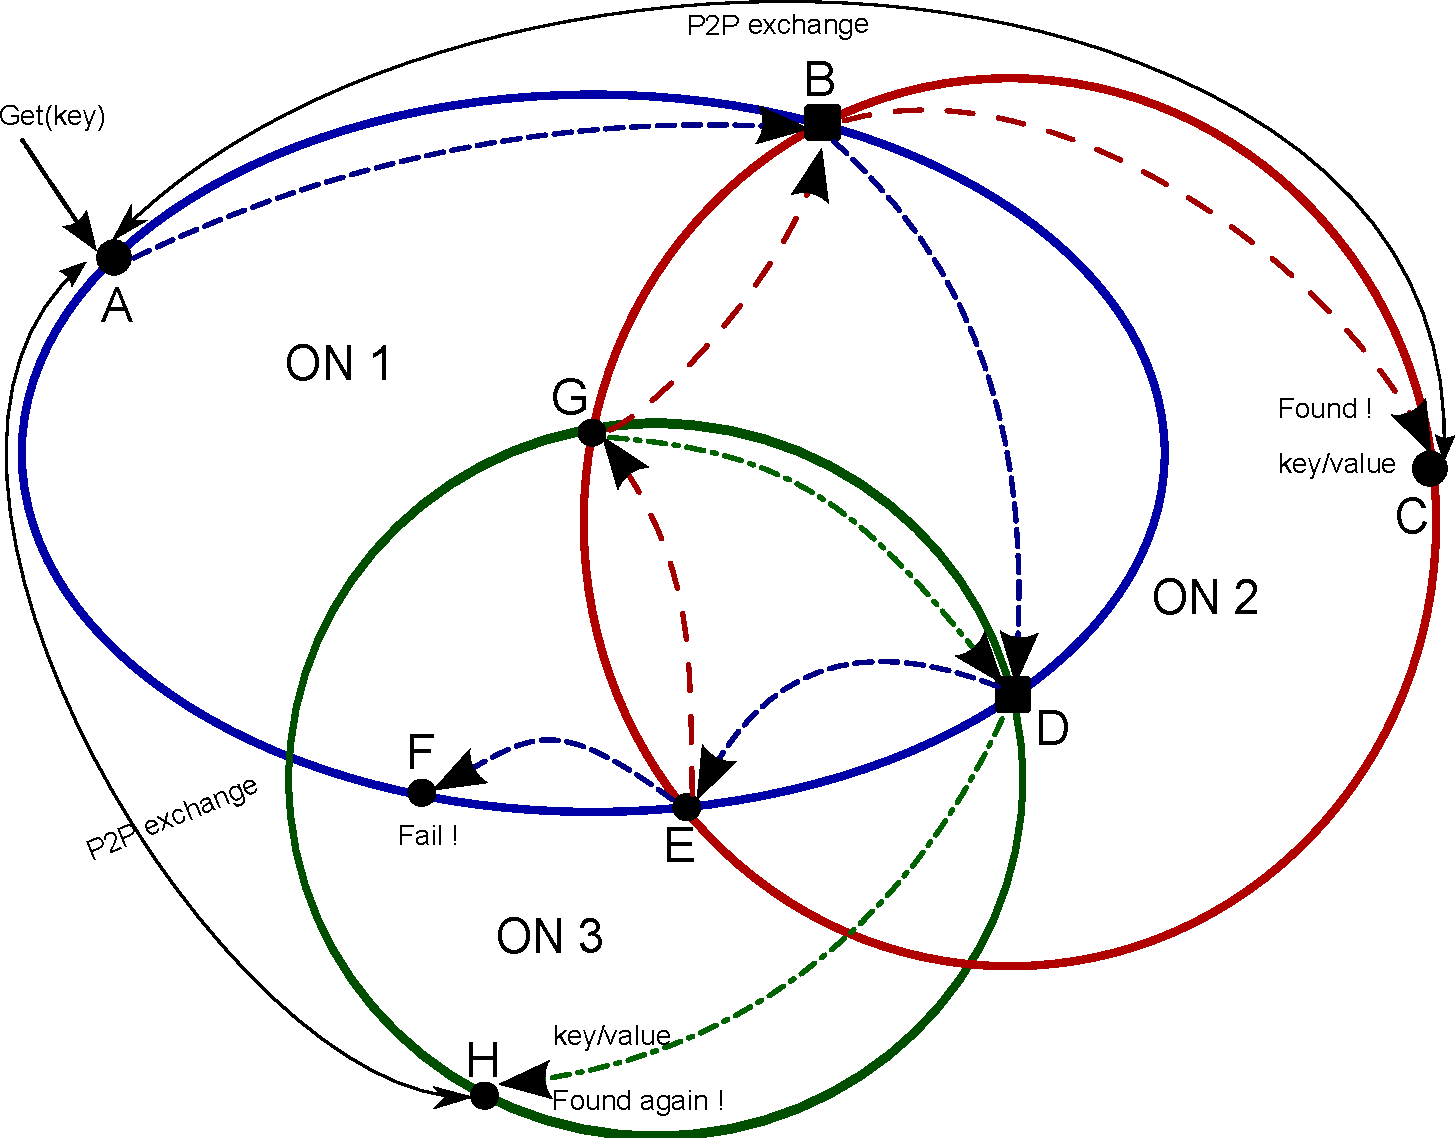
\includegraphics[width=\columnwidth]{fig/GET_into_other_ON.pdf}
  \caption{Routing across differents overlays\label{fig:example}}
  \end{figure}



  \begin{figure}
    \centering
    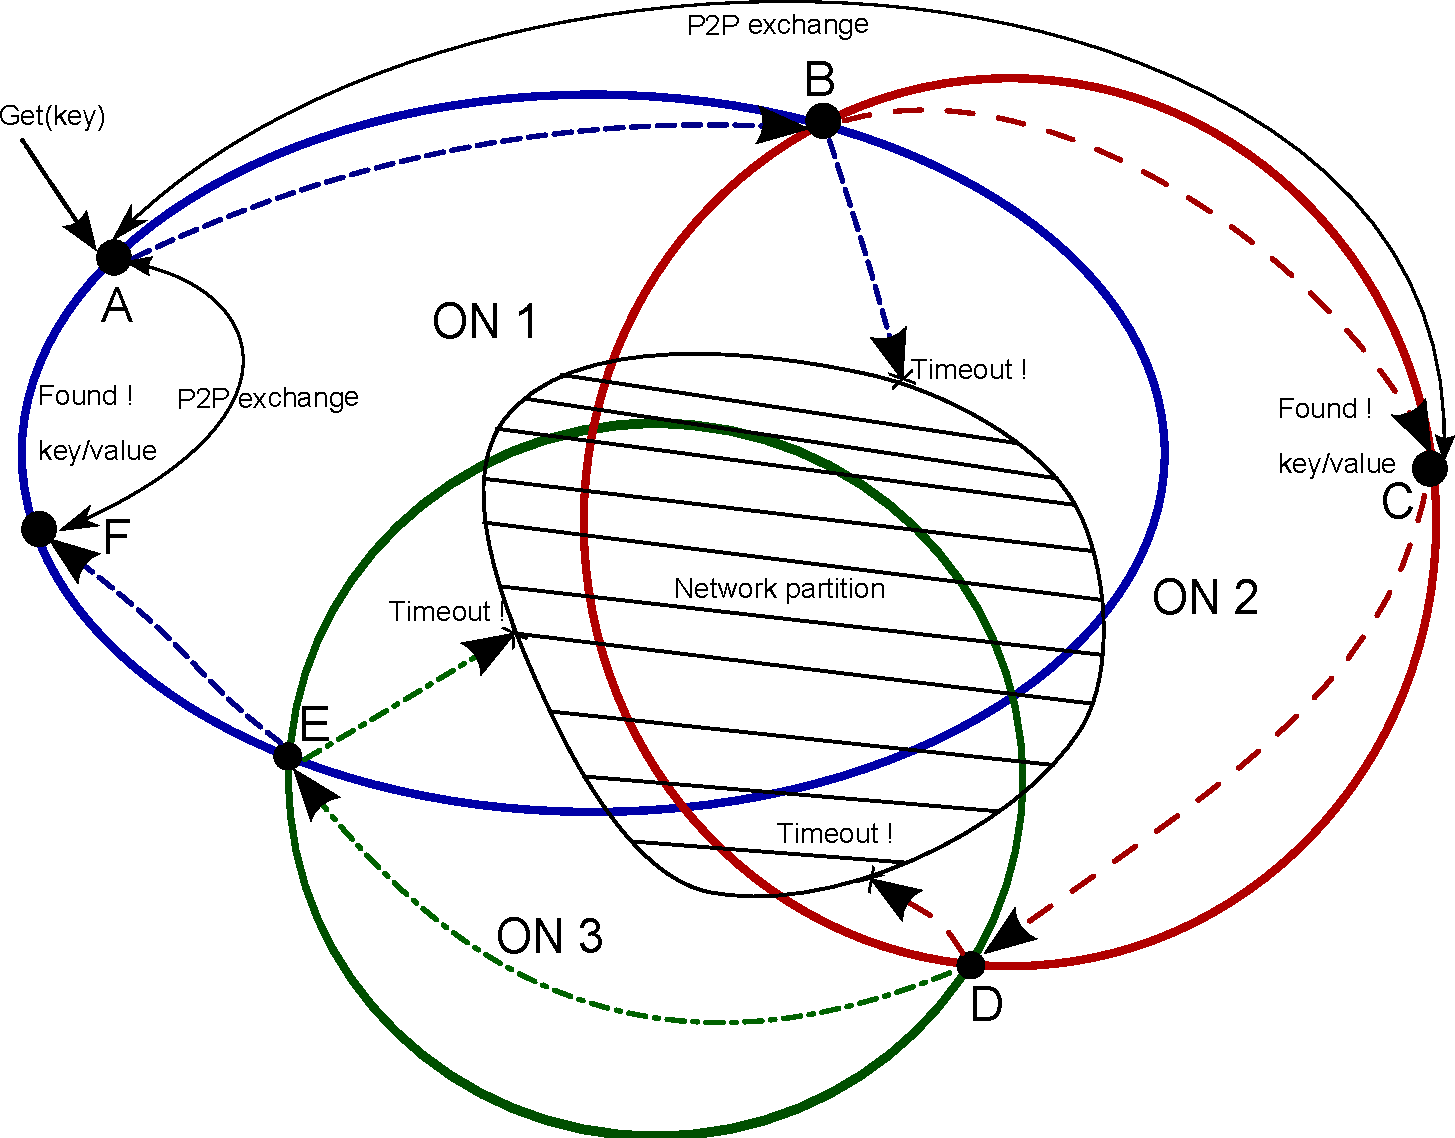
\includegraphics[width=\columnwidth]{fig/ON_with_network_partition.pdf}
    \caption{Dealing with a network partition \label{fig:example2}}
  \end{figure}


%% heart of the description
\subsection{Algorithms}
%
Figure~\ref{fig:lookup} presents the pseudo-code of the protocol using
message passing paradigm.

\subsubsection{The \texttt{GET} operation}
%
The {\tt GET} operation consists in finding the value of an object we
are seeking, provided its key. A node seeking an object sends an
\texttt{OPE(GET,key,\_)} message to an arbitrary node it knows. On
receipt (see lines~\ref{alg:ope}-\ref{alg:ope_end}), the node
generates a new tag {\tt tag} for this request that will be associated
with the query all along its path. The routing is then initiated with
a given TTL by sending an auxiliary {\tt FIND} message for this
request to the node itself; this message seeks the node(s) responsible
for the key sought in order to read the value (if it exists).

On receipt of a {\tt FIND} message (see
lines~\ref{alg:find}-\ref{alg:find_end}), the node checks the TTL and
the tag of the request before starting processing the request, and,
first, recording it as \emph{already processed} (``game over''
stategy). The retrieval process starts then locally, in two steps for
each intra-overlay the node belongs to: $(i)$ it checks if, according
to the particular retrieval algorithm of the intra-overlay, it is
itself assigned a range of keys containing {\tt key} (line
\ref{alg:test}), if this is the case, for this overlay, the retrieval
process ends and a {\tt FOUND} message is sent back to the initiator
of the request informing it that the potential value sought is stored
on this node (line~\ref{alg:send_found})). $(ii)$ if the node was not
responsible for the key in this particular overlay, it forwards the
request to the \emph{next hop} inside this intra-overlay, according to
the particular overlay's policy (line \ref{alg:find_end}).

% \Fr{}\Ce{ Parler de {\tt distrib\_mrr} as the function calculating the
% associative list ({\tt net-mrr}), ligne 2.04 (see web page for
% examples of how the function work)}

On receipt of such a {\tt FOUND} message --- recall that several
responses can be obtained for a request --- the initiator of the {\tt
  GET} request sends a {\tt READ\_TABLE} message to the responsible of
the key, basically to get the value of the key sought (see
lines~\ref{alg:get_code}-\ref{alg:get_code_end}).

\subsubsection{The \texttt{PUT} operation}
%
The {\tt PUT} operation is a declaration of a resource. Depending on
the purpose of the resource aggregation, the {\tt PUT} policy may
change:

\begin{itemize}
 \item If the purpose of the aggregation is to let each overlay keep
   the control on their information (with exclusive rights for
   writing and updating the information) while letting nodes from
   other overlay read this information, the {\tt PUT} operation will
   be performed independently within each overlay, each node
   declaring their resources to their intra-overlays. In this first
   case, the {\tt PUT} operation will not be different as in a set of
   intra-overlays without inter-connection, and corresponds to set
   the Maximum-Replication-Rate (MRR) to 0.

 \item If the purpose of the aggregation is to build a globally
   distributed information system, each node may declare its resources
   to a set of intra-overlays it may not belong to. In this last case,
   the {\tt PUT} operation involves mechanisms very similar to the
   {\tt GET} operation and the Maximum-Replication-Rate (MRR)
   different than zero tells how many copies we want to distribute in
   the inter-overlay. Line $2.04$ computes via the function {\tt
     distrib\_mrr}\footnote{Please refer to the Synapse web page for
     more information} the required values of MRR for a {\tt PUT}
   request, starting from both its current value and the number of
   intra-overlays the request will be forwarded to. Recall that MRR is
   ignored when the message is not a {\tt PUT} operation. In fact, a
   node declaring a resource will also seek nodes in the Synapses
   responsible for their resources. Once such location is found
   (similarly than for the {\tt GET} operation), the initiator of the
   request has just to send the value to be stored by the responsible
   nodes found. This is achieved by
   lines~\ref{alg:put_code}-\ref{alg:put_code_end}.

\end{itemize}

\subsubsection{The \texttt{JOIN} and \texttt{INVITE} operations}
%
The {\tt JOIN} message is sent by a node entering the network, upon a
reception of an {\tt INVITE} message. Please refer to
lines~\ref{alg:join_req}-\ref{alg:join_req_end} for invitation, and to
lines~\ref{alg:join_req_ok}-\ref{alg:join_req_ok_end} for join. The
intra-overlays in which a joining node will act can be chosen in
different ways. A peer receiving an invitation to join a network
through the {\tt INVITE} message sent by another node can evaluate,
via the {\tt good\_deal?}  social-based primitive, the relevance of
this invitation. If the invitation was positively evaluated, it can
send a {\tt JOIN} message to the peer that launched the
invitation. Upon receipt of a {\tt JOIN} message, a peer can decide,
again via the {\tt good\_deal?}  primitive, whether or not this join
is interesting for it.


% \paragraph{The \texttt{leave} operation.}

% The {\tt leave} operation differs from the others in the sense that no
% additional code is required, each leaving operation being normally
% handled by each overlay a node belongs to.



\up{3}
\section{The Simulations\label{sec:simulations}}
\up{3}
% simulation.tex
The purpose of the simulations is to allow for better understanding of
the behavior of platforms interconnecting structured overlay networks
through the Synapse approach. We focus on the key metrics
traditionally considered in distributed information retrieval process,
such as exhaustiveness (the extent of existing objects effectively
retrieved by the protocol), latency (number of hops required to reach
the requested object) and the amount of communications produced
(number of messages generated for one request). We want to highlight
the behavior of these metrics while varying the topology (the number
of synapses and their connectivity, TTL, the number of intra-overlays
...).

%\subsection{Settings}
%
\noindent{\bf Settings.}
%
Our simulations have been conducted using Python scripts, and using
the \emph{white box} protocol, capturing the essence of the Synapse
approach. The topology of the overlay simulated is a set of Chord
networks interconnected by some synapses.  Information is a set of
{\tt (key,value)} pairs. Each pair is unique and exists once and only
once in the network. We study the unstructured interconnection of
structured networks. We used discrete-time simulation: queries are
launched on the first discrete time step, initiating a set of messages
in the network, and each message sent at the current step will be
received by its destination (next routing hop) at the next hop.

%\subsection{Synapses}
%
\noindent{\bf Synapses.}
%
Our first set of simulations has the intent of studying how the
previously mentioned metrics vary while we add synapses or increase
the degree of existing ones (the number of intra-overlays a co-located
node belongs to). The number of nodes was fixed to $10000$, uniformly
distributed amongst $20$ overlays (approximately $500$ nodes within
each Chord). Queries are always triggered by one random node, the key
sought by a query is also picked uniformly at random among the set of
keys stored by the network. A query is said to be \emph{satisfied} if
the pair corresponding to the key has been successfully retrieved.

We first studied search latency, \ie\ the number of hops to obtain the
first successful response.
% (if the keys searched were stored on several overlays, the latency
% would correspond to the first response received).
As illustrated in Figure~\ref{fig:3D-hops}, one first point to notice
is that the number of hops remains logarithmic when changing a Chord
network into a Synapse network (the number of nodes is $10000$, the
latency never exceeds 14). Other experiments conducted by increasing
the number of nodes confirm this. More precisely,
Figure~\ref{fig:3D-hops} (left) highlights the following behavior:
$(i)$ when the network contains only a few synapses, the latency first
increases with the degree of synapses: only a few \emph{close} keys
are retrieved (keys available in the network of the node that
initiated the query); $(ii)$ then, when both parameters (the
connectivity and the number of synapses) have reached a certain
threshold, the searches can touch more synapses, and the whole network
becomes progressively visible, multiple parallel searches become more
and more frequent and distant nodes (and keys) are reached faster. As
we can see, increasing the number of synapses decreases the latency of
only a small constant factor. In other words, synapse topologies does
not need a lot of synapses to be efficient. This result fits with
random graphs behavior: when the number of neighbors in the graph
reaches a (small) threshold, the probability for the graph to be
connected tends towards $1$.
% 
\begin{figure}[!t]
\up{4}
        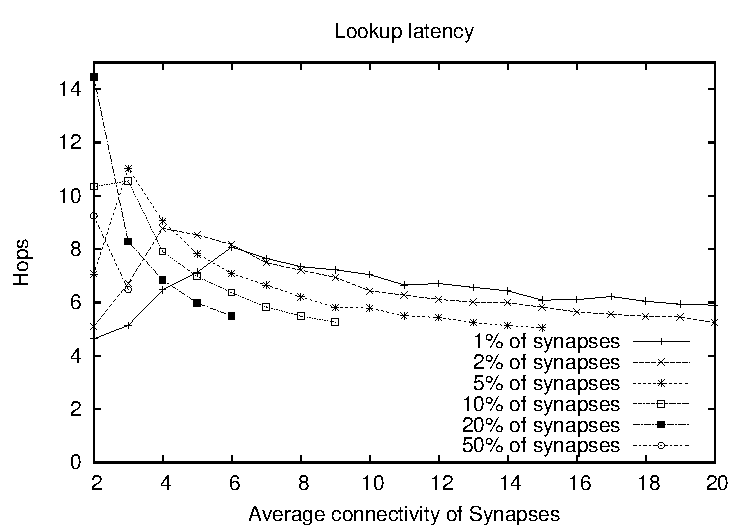
\includegraphics[width=0.5\linewidth]{fig/3D-hops.pdf}
        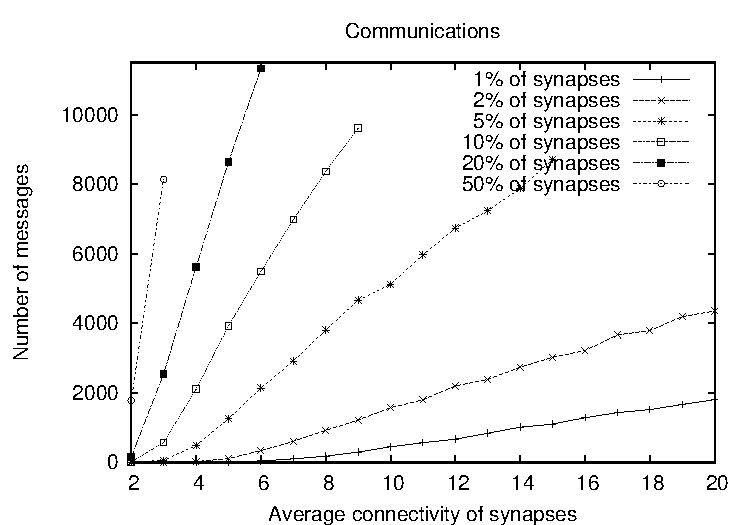
\includegraphics[width=0.5\linewidth]{fig/3D-msgs.pdf}
\up{4}
        \caption{Latency and communications in Synapse\label{fig:3D-hops}}
%\up{2}
\end{figure}
%
Obviously, multiple searches in parallel lead to an increased number
of messages. As illustrated in Figure~\ref{fig:3D-hops} (right), this
number increases proportionally with the connectivity and the number
of synapses. 
% A good-deal strategy in synapses can leverage this inter-network
% overhead.

% Moreover, the number of total communications tends to be linear in
% the number of nodes, which can obviously become a serious problem,
% as pointed out in unstructured networks.
%
% \begin{figure}
%   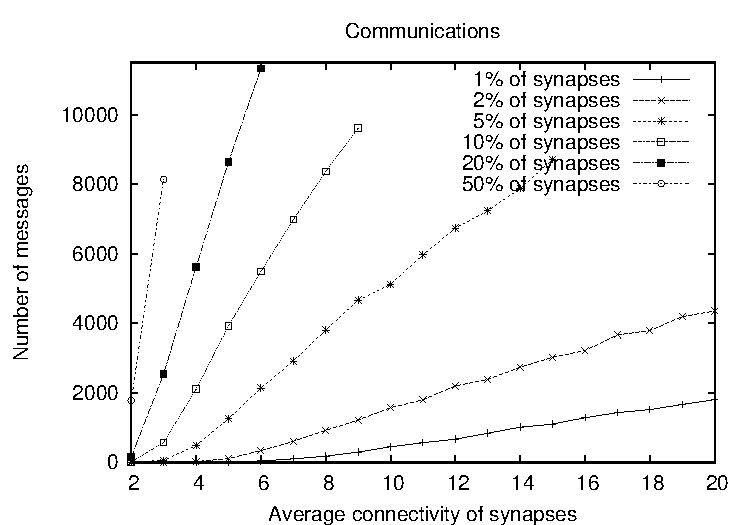
\includegraphics[width=0.5\linewidth]{fig/3D-msgs.pdf}
%   \caption{Synapses and communicationss\label{fig:3D-msgs}}
% \end{figure}

%%% TTL simulations

%\subsection{Time-To-Live}
%
\noindent{\bf Time-To-Live.}
As we pointed out, the number of messages can become high when the
number of synapses increases. To limit this impact, we introduced a
Time-to-Live (TTL) to reduce the overhead while keeping an acceptable
level of exhaustiveness.  We launched a second set of experiments in
order to study the impact of the TTL on the search queries. This TTL
is simply decreased every time the query traverses a node. 

The purpose is here is to preserve significant exhaustiveness, while
reducing the amount of communications undergone by the
inter-overlay. We made the number of overlays vary, to experiment the
impact of the \emph{granularity} of the network.  In other words, a
Synapse network made of few large structured intra-overlays could be
called \emph{strongly structured}, while another network with many
smaller structured intra-overlays could be called \emph{weakly
  structured}. The number of nodes was still set to $10000$, and every
node is a synapse belonging to $2$ overlays chosen uniformly at
random.


\begin{figure}[!t]
  \up{4}
  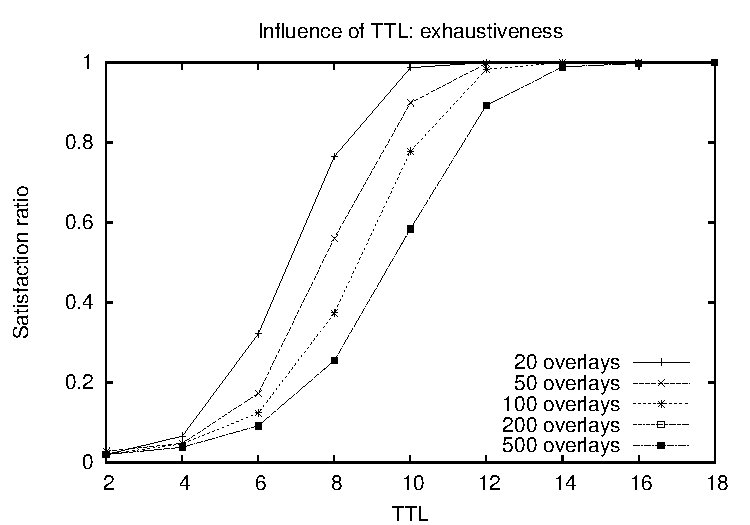
\includegraphics[width=0.5\linewidth]{fig/TTL-sat.pdf}
  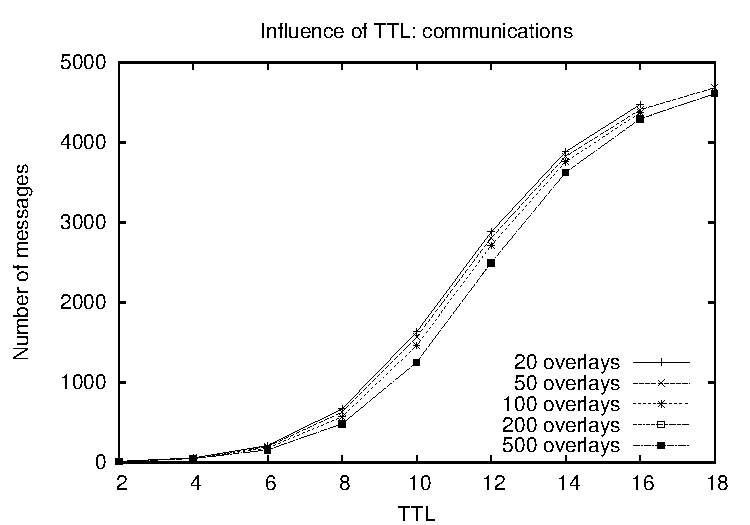
\includegraphics[width=0.5\linewidth]{fig/TTL-msgs.pdf}
  \up{4}
  \caption{TTL \vs\ exhaustiveness and communications\label{fig:TTL-sat}}
  \up{4}
\end{figure}
% 
% \begin{figure}
%   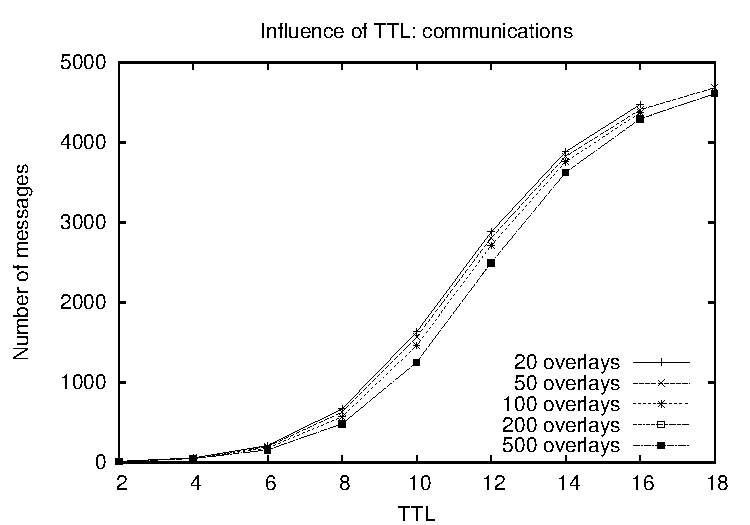
\includegraphics[width=0.45\linewidth]{fig/TTL-msgs.pdf}
%   \caption{TTL and communications\label{fig:TTL-msgs}}
% \end{figure}
%  
Figure~\ref{fig:TTL-sat} (left) confirms that a low synapse degree
($2$) is enough to achieve quasi-exhaustiveness. Another interesting
result is that TTL can be bounded without any impact on the
exhaustiveness ($10$ or $12$ is enough even when the number of
overlays interconnected is $500$), while, as highlighted by
Figure~\ref{fig:TTL-sat} (right), drastically reducing the amount of
communications experienced, with the number of messages being almost
divided by $2$. To sum up, Synapse architectures can use TTL, leading
to a significant exhaustiveness while drastically reducing the
expected overhead.
%
Finally, still see Figure~\ref{fig:TTL-sat}, the \emph{granularity}
(defined above) does not significantly influence exhaustiveness and
communications when the number and connectivity of the synapses are
fixed.

%\subsection{Connectivity and Peers' churn}
%
\noindent{\bf Connectivity and Peers' churn}
%
Figure~\ref{fig:3D-sat} (left) shows the evolution of the
exhaustiveness while increasing the average number of overlays a
synapse belongs to. We repeated the experiment for different ratios of
synapses (in percentage of the total number of nodes). The
exhaustiveness is improved by increasing both factors. We obtain more
than 80\% of satisfaction with only 5\% of nodes belonging to 10
floors, and other nodes belonging to only one intra-overlay. When each
node belongs to $2$ overlays, the exhaustiveness is also almost
guaranteed.

\begin{figure}[!t]
  \up{4}
  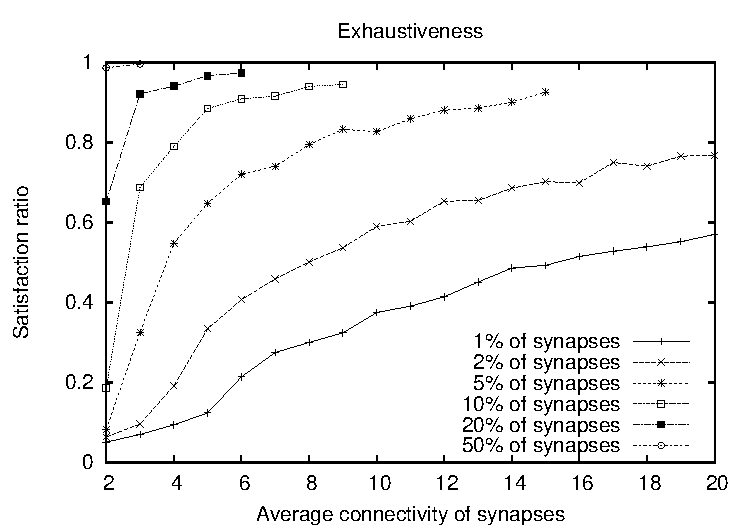
\includegraphics[width=0.5\linewidth]{fig/3D-sat.pdf}
  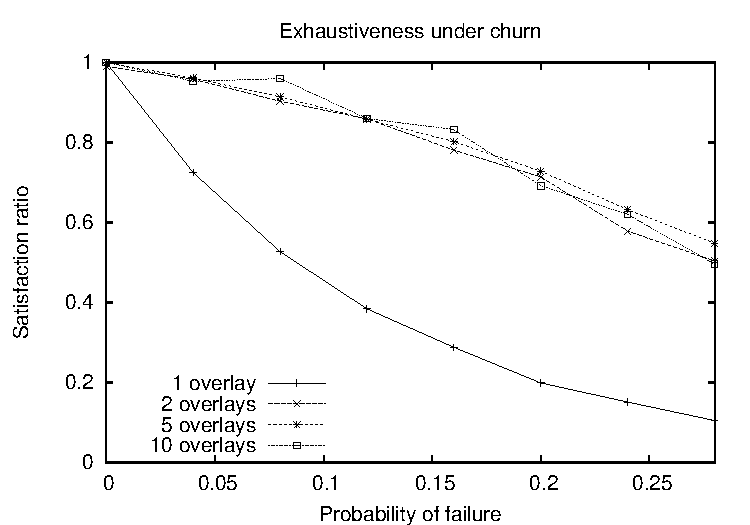
\includegraphics[width=0.5\linewidth]{fig/churn-sat.pdf}
  \up{4}
  \caption{Exhaustiveness \vs\ synapses and churn\label{fig:3D-sat}}
  \up{4}
\end{figure}
%
Since networks are intended to be deployed in a dynamic settings (nodes
joining and leaving the network without giving notice), we conducted a
final set of simulations to see the tolerance of Synapse compared to a
single Chord overlay network. In other words, the question is
\emph{Does an interconnection of small Chords better tolerate
  transient failures than one large unique Chord?} In this experiment,
at each step, a subset of nodes is declared unreachable (simulating
the churn), making message routing fail. As we can see on
Figure~\ref{fig:3D-sat} (right), improvement on the number of
satisfied requests can be obtained through a Synapse network: when the
probability of failure/disconnection of a node increases, the global
availability of the network is far less reduced with Synapse than with
Chord. This shows that such synapse architectures are more robust and
thus good candidates for information retrieval on dynamic platforms.
 
\section{The Experimentations\label{sec:deployement}}
\up{3}

\subsection{JSynapse}

In order to test our protocols on real platforms, we have first
developed JSynapse, a Java-based software prototype, which uses Java
RMI standard for communications between nodes, and whose purpose is to
capture the very essence of our Synapse protocol. It is a flexible and
ready to be plugged library which can inter-connect any type of
overlay networks.  This prototype fully implements a Chord-based
inter-overlay network along with our original Maximum Replication Rate
mechanism. It is a lightweight easy to extend software. We also
provided some practical classes which help in automating the generation
of the inter-overlay network and the testing of specific scenarios.

We have experimented JSynapse on the Grid'5000 platform connecting
more than $20$ clusters on 9 different sites. Again, Chord was used as
the intra-overlay protocol.

In our first deployments, we used one cluster located at Sophia
Antipolis, France. The {\tt Helios} cluster is made of $56$ quad-core
AMD Opteron 275 linked by a gigabit Ethernet connection. The Synapse
network created was first made of up to $50$ processors uniformly
distributed among $3$ Chord intra-overlays. Then, still on the same
cluster, as nodes are quad-core, we deployed up to $3$ logical nodes
by processor, thus creating a $150$ nodes overlay network, nodes being
dispatched uniformly over $6$ overlays. During the deployment,
overlays were progressively bridged by synapses (whose
degree was always $2$).

Our goal is here to give a proof of concept and to show the viability
of the Synapse approach while confirming results obtained by
simulation. We also focused on the metrics affecting the user
(satisfaction ratio and time to get a response). In our deployment,
once his request was sent, a user waits only $1$ second before closing
channels opened to receive responses. If no response was received
after $1$ second, the query is considered as not satisfied.

Figure~\ref{dep:1-sat} shows the satisfaction ratio when increasing
the number of synapses. As expected, the general behavior is
comparable to the simulation results and a quasi-exhaustiveness is
achieved, with only a connectivity of $2$ for synapses.

\begin{figure}
        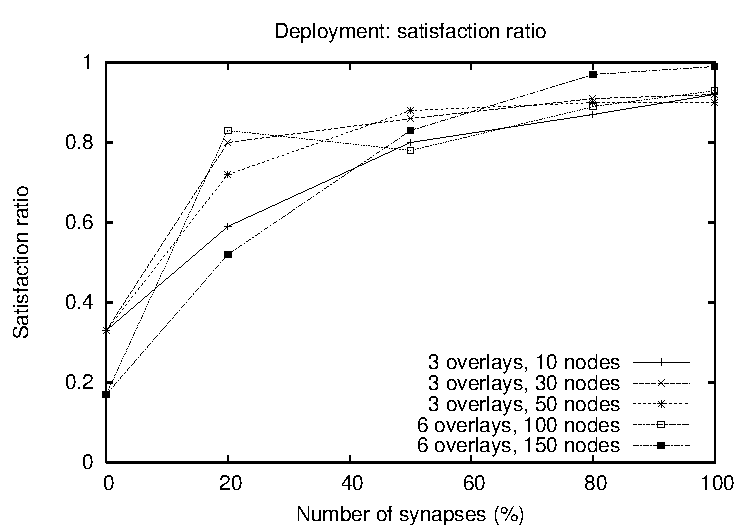
\includegraphics[width=\linewidth]{fig/dep1-sat.pdf}
        \caption{Deploying Synapse on the {\tt Helios} cluster -
        Exhaustiveness\label{dep:1-sat}}
\end{figure}

Figure~\ref{dep:1-time} illustrates the fact that, the latency
experienced by the user when launching a request is very low (few
milliseconds) even when a lot of synapses may generate a lot of
messages. Obviously this result has to be considered while keeping the
performances of the underlying hardware and network used in
mind. However, this suggests the viability of our protocols, the
confirmation of simulation results, and the efficiency of the software
developed.

\begin{figure}
        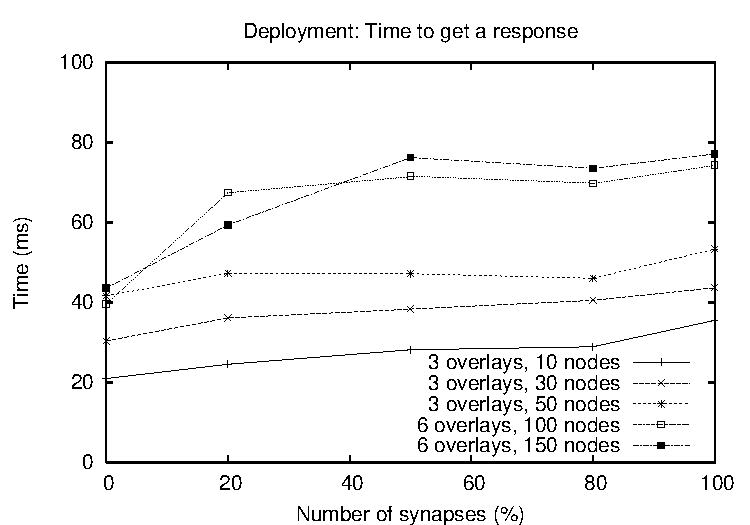
\includegraphics[width=\linewidth]{fig/dep1-time.pdf}
        \caption{Deploying Synapse on the {\tt Helios} cluster - Latency}
        \label{dep:1-time}
\end{figure}

\subsection{Open-Synapse}
%
We have also developed {\tt open-synapse}, based on the stable and
widely used {\tt open-chord} implementation, which provides a complete
and efficient Chord implementation. Open-Synapse has been developed as
an extension of the {\tt open-chord} core and thus takes advantage of
its robustness and reliability. A preliminary set of tests have been
successfully conducted on {\tt open-synapse}, involving $50$ nodes and
different randomly generated scenarii.

\up{3}
\section{Related Work\label{sec:relatedwork}}
\up{3}
% related.tex

%% Identifying future trends Independantly, authors

In \cite{siekkinen_beyondfuture_2007}
and~\cite{fonte_interdomain_2008}, authors have recently presented
some architectural issues with the Internet and identified some future
trends, one of which is the inter-communication of
\emph{realms}\footnote{A realm is a term authors use in order to
  identify a network instance.}. They emphasise on the
inter-communication of logical networks, and discuss various ways to
do so. In particular, they point out that co-existing realms should
share nodes in some cases and should not in some others. For instance,
networks may deliberately behave selfishly only aiming at the
improvement of their application-level QoS by taking advantage of
dedicated paths to other networks, \ie\ using \textit{gateways},
acting as dedicated bridges between networks. But in many cases they
argue that it is more natural to take advantage of nodes that are
already part of multiple overlay networks, \ie\ using \emph{co-located
  nodes}.

\subsection{Cooperation through hierarchy}
%% Hierarchical
Pointing out the limits of a unique global structured overlay network
(rigidity, maintenance cost, security, etc.), several propositions
have been made over the years to build alternate topologies based on
the coexistence of smaller local overlay networks. A first approach
has been based on hierarchical systems \cite{Biersack,XuMH03}, some
elected super-peers being promoted to a top-level overlay network,
leading to the requirement of costly merging mechanisms to ensure a
high level of exhaustiveness. In a more general view, merging several
co-existing structured overlay networks has been shown to be a very
costly operation \cite{Datta,Haridi}.

%% Transition/Contribution
In the context of mobile ad hoc networks, Ariwheels
\cite{BCCL08,LBCC08} has been designed to provide a large variety of
services through a multi-layer overlay network, where super-peers,
called Brokers, act as servers for a subset of peers.  Ordinary peers,
called Agents, submit queries to their Broker and receive results from
it. Ariwheels provides an efficient mapping between physical devices
in the wireless underlay network and virtual entities in the overlay
network.

\subsection{Cooperation through gateways}

Authors in~\cite{cheng2006tdh} presented two models for two overlays
to be (de)composed, known as \textit{absorption} (a sort of merging)
and \textit{gatewaying}.  Their protocol enables a CAN-network to be
completely absorbed into another one (in the case of the absorption),
and also provide a mechanism to create bridges between DHTs (in the
case of the gatewaying). They do not specifically take advantage of a
simple assumption that nodes can be part of multiple overlays in the
same time, thus playing the role of natural bridges.

More recently, authors in \cite{cheng_bridging_2007} propose a novel
information retrieval protocol, based on gateways called
\emph{DHT-gatewaying}, which is scalable and efficient across
homogeneous\footnote{Same implementation and same keysize (ex. Two
  160-bit Chord DHTs).}, heterogeneous\footnote{Same implementation
  and different keysize (ex. One 160-bit Chord and one 256-bit Chord
  DHTs).}  and assorted\footnote{Different implementation and/or
  different keysize (ex. One 160-bit Chord and one 256-CAN DHTs).}
co-existing structured overlay networks. They argue that there is not
a preferred structured overlay network implementation, and that peers
are members of co-existing DHTs. Their assumptions are $(i)$ only some
peers support the implementations of different DHTs and $(ii)$ some
peers are directly connected to peers that are members of other DHTs,
and are called \textit{Virtual Gateways (VG))}. When a request is sent
in one overlay, and no result was found, the requester can decide to
widen his search by forwarding its original search request to nodes
which belong to other structured overlay networks (mapping the search
to the format supported by their relative overlay). A TTL value is
added to the original search in order to avoid cycles; this value is
decremented each time a request crosses a new DHT
domain. Unfortunately the evaluation of their protocol lacks precious
details and precision. It is unclear how they evaluate their protocol.

%Because VGs can be overloaded, authors
%devised a mechanism in order to distribute the mapping by electing
%more VGs (according to a specific VG determination scheme), and they
%also introduced self-organizing \emph{gateways pointers} whose roles
%are to keep track of VGs where-abouts.


%% Synergy: co-located nodes are good candidates
%% compare hierarchy and gateway to our approach
%% and state why co-located nodes are a more
%% natural choice
\subsection{Cooperation through co-located nodes}
%% Cooperation: more hints

Authors in \cite{kwon_synergy:overlay_2005} present Synergy, an
overlay inter-networking architecture which improves the routing
performance in terms of delay, throughput and packet loss by providing
cooperative forwarding of flows between networks. Authors suggest that
co-located nodes are good candidates for enabling inter-overlay
routing and that they reduce traffic. Our approach can be also seen as
a deeper study of their concepts.

On the way of designing inter-overlay networking based on co-located
nodes, authors in~\cite{junjiro_design_2006} present algorithms which
enable the symbiosis between different overlays networks with a
specific application in mind: file sharing. They propose mechanisms
for hybrid P2P networks cooperation and investigates the influence of
system conditions such as the numbers of peers and the number of
meta-information a peer has to keep. They provide interesting
observations on how to join a candidate network, cooperative peers'
selection, how to find other P2P networks, when to start cooperation,
by taking into account the size of the network (for instance a very
large network will not really benefit from a cooperation with a small
network), so on and so forth. Again, a more comprehensive
understanding of this approach is missing.

%Their simulations showed the effect of
%the popularity of a cooperative peer on the search latency evaluation,
%that is the more a node has neighbors, the better, as well as the
%effect of their caching mechanism which reduces (when appropriately
%adjusted) the load on nodes (but interestingly does not contribute to
%faster search).

%% Focus on internetwork routing policies

Authors in \cite{furtado_multiple_2007} consider multiple spaces with
some degree of intersection between spaces, \ie\ with co-located
nodes. They focused on different potential strategies to find a path
to another overlay from a given overlay, \ie\ how requests can be
efficiently routed from one given overlay to another one. They
compared various inter-space routing policies by analyzing which
trade-offs, in terms of state overhead, would give the best results,
in terms of the number of messages generated and routed, the number of
hops it takes to find a result and the state overhead (\ie\ the number
of fingers a node has to keep). They provide a comparative analytical
study of the different policies. They showed that with some dynamic
finger caching and with multiple gateways (in order to avoid
bottlenecks and single points of failures) which are tactfully laid
out, they attain pretty good performances. Their protocol focus on
DHTs interconnection, we extend it to any kind of overlays.

%% Babelchord
In our previous preliminary work \cite{LTB09}, we introduced
BabelChord, a protocol for inter-connecting Chord overlay networks
using co-located nodes that are part of multiple Chord
``floors''. These nodes connect, in an unstructured fashion, several
Chord overlays together The simulations showed that we could achieve
pretty high exhaustivity with a small amount of those co-located
nodes. Our current paper, in turn, focuses on the co-located nodes
heuristic in far more details than the aforementioned work by
providing not only a more generic protocol which enables inter-overlay
routing that can in principle be applied to connect arbitrary
heterogeneous overlays, but also more simulations to show the
behaviours of such networks as well as a real implementations and live
experiments.



% \subsection{Most related works }

% The most related works that can be compared to the current paper are:
% \cite{cheng_bridging_2007,kwon_synergy:overlay_2005,furtado_multiple_2007,
% junjiro_design_2006,LTB09}.
% In summary the key differences/similitudes with the present paper are:

% \begin{maliste}
% % \item \cite{cheng_bridging_2007}: Authors here present a protocol
% % which can handle co-located nodes as well as direct gateways. Although they
% % focus on wireless ad hoc  network, they claim that their protocol can
% % be used in wired networks too. Their insights  regarding the placement
% % and the selection of their \textit{Virtual Gateways} are fairly
% % precise.  Unfortunately the evaluation of their protocol lacks
% % precious details and precision. It is unclear  how they evaluate their
% % protocol.

% \item \cite{kwon_synergy:overlay_2005}: The Synergy internetworking
% architecture  also makes use of co-located node in order to improve
% global performances. They try to create and maintain long-lived flows
% (\ie long-lived paths) that can be used to cross  overlay
% boundaries. They provide hints on how to choose nodes which will take
% part in those flows,  and they provide simulations and real experiments from a
% prototype client.  However they do not go into details as much as we
% do in this paper regarding the algorithms that enable such overlay
% inter-connection.

% \item \cite{furtado_multiple_2007}: The authors strongly focused their
% attention  on the state overhead of the nodes participating in several
% spaces in the same time (\ie using also co-located nodes),
% and provide fairly accurate analyses and strategies to
% minimise it. They do not provide a generic protocol in the sense that
% their protocol only focus on DHT's inter-connection.

% \item \cite{junjiro_design_2006}: Authors only focus on file sharing
% whereas our protocol can be applied to any application. Even if the
% algorithms and the various observations they present are relevant
% they fail to provide any real experiments nor an in-depth analysis of
% their algorithms.

% \item \cite{LTB09}: Our current paper focuses on the co-located
% nodes heuristic in more details than the aforementioned work by
% providing not only a more generic protocol which enables
% inter-overlay routing that can in principle be applied to connect
% arbitrary heterogeneous overlays, but also more simulations to show the
% behaviours of such networks as well as a real implementation and live
% experiments.

% \end{maliste}


%  We based our work on co-located nodes and
% try to take advantage of the fact that a node participates in multiple
% overlay networks in the same time on the Internet. However, we try to
% provide a deeper analysis of such type of inter-overlay networks
% compared to other works and we also try to not only to give strong
% simulations but also live deployments.


%% add a proper conclusion

\begin{comment}
  In this sense, and in response to overlay detractors, we argue
  %% list some coherent responses for their comments that ON are not
  %% suited for interconnecting domains
  that works like \cite{XuMK03}, \cite{EURECOM+1205} and \cite{zhou_balancing_2003} show efficient method for constructing an overlay network while taking into account the underlying topology. Therefore we can say with confidence that we do have mechanisms in order to ensure that the paths the packets traverse are not using duplicate physical links.
\end{comment}





\up{3}
\section{Conclusion}
\up{3}
% conclusions.tex

We have introduced Synapse, a scalable protocol for information
retrieval in heterogeneous inter-connected overlay networks relying on
co-located nodes.  Synapse is a generic and flexible
\emph{meta}-protocol which provides simple mechanisms and algorithms
for easy overlay networks' interconnection. We have given the set of
algorithms behind our protocols and provided a set of simulations
allowing to capture the behavior of such networks and shows their
relevance in the context of information retrieval, using key metrics
of distributed information retrieval. We have also developed {\tt
JSynapse}, a lightweight implementation of Synapse, and experimented
it on the Grid'5000 platform, thus confirming our simulation and
giving a proof of concept of our protocol.

As future work, we first intend to focus on social mechanisms involved
in synapses, which can greatly influence the shape of the network. On
the practical side, we plan to extend {\tt JSynapse} and plug in some
other overlay network implementations. More intensive tests and
deployments of {~\tt{open-synapse}}, our early prototype based on {\tt
open-chord} will also be considered.


% \bigskip
% \noindent{\bf Acknowledgment}
% The authors warmly thank Ernst Biersack for the precious help in
% reading an early version of this paper.  \bibliographystyle{plain}
% \bibliography{biblio}
 
%\up{2}
\begin{thebibliography}{10}
%\up{1}
{\scriptsize
\bibitem{BCCL08}
D.~Borsetti, C.~Casetti, C.~Chiasserini, and L.~Liquori.
\newblock {\em Heterogeneous Wireless Access Networks: Architectures and
  Protocols}, chapter {Content Discovery in Heterogeneous Mobile Networks}.
\newblock Sringer-Verlag, 2009.

\bibitem{castro_scribe:large-scale_2002}
M.~Castro, P.~Druschel, A.-M. Kermarrec, and A.~Rowstron.
\newblock {SCRIBE: A Large-Scale and Decentralized Application-Level Multicast
  Infrastructure}.
\newblock {\em {IEEE} Journal on Selected Areas in Communications {(JSAC)}},
  20, 2002.

\bibitem{cheng_bridging_2007}
L.~Cheng.
\newblock {Bridging Distributed Hash Tables in Wireless {Ad-Hoc} Networks}.
\newblock In {\em Global Telecommunications Conference, 2007. {GLOBECOM} '07.
  {IEEE}}, pages 5159--5163, 2007.

\bibitem{cheng2006tdh}
L.~Cheng, R.~Ocampo, K.~Jean, A.~Galis, C.~Simon, R.~Szabo, P.~Kersch, and
  R.~Giaffreda.
\newblock {Towards Distributed Hash Tables (De) Composition in Ambient
  Networks}.
\newblock {\em LNCS}, 4269:258, 2006.

\bibitem{Datta}
A.~Datta and K.~Aberer.
\newblock The\,challenges\,of\,merging\,two\,similar\,structured\,overlays:\,{A}\,tale\,of\,two\,networks.\,In\,{\em IWSOS},\,2006.

\bibitem{Biersack}
L.~G. Erice, E.~W. Biersack, K.~W. Ross, P.~A. Felber, and G.~U. Keller.
\newblock {Hierarchical P2P Systems}.
\newblock In {\em Euro-Par}, 2003.

% \bibitem{fonte_interdomain_2008}
% A.~Fonte, M.~Curado, and E.~Monteiro.
% \newblock {Interdomain Quality of Service Routing: Setting the Grounds for the
%   Way Ahead}.
% \newblock {\em Annals of Telecommunications}, 63(11):683--695, 2008.

\bibitem{furtado_multiple_2007}
P.~Furtado.
\newblock {Multiple Dynamic Overlay Communities and Inter-space Routing}.
\newblock {\em LNCS}, 4125:38, 2007.

\bibitem{junjiro_design_2006}
K.~Junjiro, W.~Naoki, and M.~Masayuki.
\newblock {Design and Evaluation of a Cooperative Mechanism for Pure P2P
  File-Sharing Networks}.
\newblock {\em {IEICE} Trans Commun {(Inst} Electron Inf Commun Eng)},
  {E89-B}(9):2319--2326, 2006.

\bibitem{kwon_synergy:overlay_2005}
M.~Kwon and S.~Fahmy.
\newblock {Synergy: an Overlay Internetworking Architecture}.
\newblock In {\em Proc. of International Conference on Computer Communications
  and Networks}, pages 401--406, 2005.

\bibitem{LBCC08}
L.~Liquori, D.~Borsetti, C.~Casetti, and C.~Chiasserini.
\newblock {An Overlay Architecture for Vehicular Networks}.
\newblock In {\em IFIP Networking, International Conference on Networking},
  volume 4982 of {\em LNCS}, pages 60--71. Springer, 2008.

\bibitem{LTB09}
L.~Liquori, C.~Tedeschi, and F.~Bongiovanni.
\newblock {BabelChord: a Social Tower of DHT-Based Overlay Networks}.
\newblock In {\em 14th Symposium on Computers and Communications (ISCC 2009)}.
  IEEE, 2009.
\newblock Short paper.

\bibitem{CAN}
\mbox{S.\,Ratnasamy,\,P.\,Francis,\,M.\,Handley,\,R.\,Karp,\,and\,S.\,Shenker.\,{A\,Scalable\,Content{-}Adressable\,Network}.\,In\,{\em SIGCOMM},\,2001.}

\bibitem{Pastry}
A.~Rowstron and P.~Druschel.
\newblock {Pastry: Scalable, Distributed Object Location and Routing for
  Large-Scale Peer-To-Peer Systems}.
\newblock In {\em Int. Conference on Distributed Systems Platforms
  (Middleware)}, 2001.

\bibitem{Haridi}
T.~M. Shafaat, A.~Ghodsi, and S.~Haridi.
\newblock Handling network partitions and mergers in structured overlay
  networks.
\newblock In {\em Proc. of P2P}, pages 132--139. IEEE Computer Society, 2007.

% \bibitem{siekkinen_beyondfuture_2007} M.~Siekkinen, V.~Goebel,
%   T.~Plagemann, {K.-A.} Skevik, M.~Banfield, and I.~Brusic.
%   \newblock {Beyond the Future Internet--Requirements of Autonomic
%     Networking Architectures to Address Long Term Future Networking
%     Challenges}.  \newblock In {\em International Workshop on Future
%     Trends of Distributed Computing Systems}, pages 89--98, 2007.

\bibitem{Chord}
I.~Stoica, R.~Morris, D.~Karger, M.~Kaashoek, and H.~Balakrishnan.
\newblock {Chord: A Scalable Peer-to-Peer Lookup service for Internet
  Applications.}
\newblock In {\em ACM SIGCOMM}, pages 149--160, 2001.
\bibitem{XuMH03} Z.~Xu, R.~Min, and Y.~Hu.  \newblock {HIERAS: A DHT
    Based Hierarchical P2P Routing Algorithm.}  \newblock In {\em
    ICPP}, 2003.  
%
}
\end{thebibliography}
 
 


% \appendix
  
% \begin{center}

% {\Large Referees can found the Synapse protocol code on}
% \bigskip

% \url{http://www-sop.inria.fr/teams/lognet/synapse/appendix}
% \end{center}


%
%% heart of the description

%%%%%%%%%%%%%
\section{``White box'' Synapse protocol }
%
Figure~\ref{fig:lookup} presents the pseudo-code of the protocol using
message passing paradigm. 


 
\subsection{The \texttt{GET} operation}
%
The {\tt GET} operation consists in finding the value of an object we
are seeking, provided its key. A node seeking an object sends an
\texttt{OPE(GET,key,\_)} message to an arbitrary node it knows. On
receipt (see lines~\ref{alg:ope}-\ref{alg:ope_end}), the node
generates a new tag {\tt tag} for this request that will be associated
with the query all along its path. The routing is then initiated with
a given TTL by sending an auxiliary {\tt FIND} message for this
request to the node itself; this message seeks the node(s) responsible
for the key sought in order to read the value (if it exists). Upon
receipt of a {\tt FIND} message, a node checks first if the TTL is
valid and second if this query was already processed on the node: in
both cases, the routing aborts, in order to avoid useless message
overhead.

% tech white 
%
% More precisely, the initialization of a search query is done via the
% following steps: The initiator $(i)$ logs the message in the node,
% $(ii)$ sets a TTL and $(iii)$ launches a {\tt FIND} message in a
% first overlay. Upon receipt of a {\tt FIND} message, a node checks
% first if the TTL is valid and second if this query was already
% processed on the node: in both cases, the routing aborts, in order
% to avoid useless message overhead.



On receipt of a {\tt FIND} message (see
lines~\ref{alg:find}-\ref{alg:find_end}), the node checks the TTL and
the tag of the request before starting processing the request, and,
first, recording it as \emph{already processed} (``game over''
strategy). The retrieval process starts then locally, in two steps for
each intra-overlay the node belongs to: $(i)$ it checks if, according
to the particular retrieval algorithm of the intra-overlay, it is
itself assigned a range of keys containing {\tt key} (line
\ref{alg:test}); if this is the case, for this overlay, the retrieval
process ends and a {\tt FOUND} message is sent back to the initiator
of the request informing it that the potential value sought is stored
on this node (line~\ref{alg:send_found}). $(ii)$ if the node was not
responsible for the key in this particular overlay, it forwards the
request to the \emph{next hop} inside this intra-overlay, according to
the particular overlay's policy (line \ref{alg:find_end}).

% \Fr{}\Ce{ Parler de {\tt distrib\_mrr} as the function calculating the
% associative list ({\tt net-mrr}), ligne 2.04 (see web page for
% examples of how the function work)}

On receipt of such a {\tt FOUND} message --- recall that several
responses can be obtained for a request --- the initiator of the {\tt
  GET} request sends a {\tt READ\_TABLE} message to the responsible of
the key, basically to first to check if any value is assigned to this
key and then to retrieve the value(s) and then get the value of the
key sought (see lines~\ref{alg:get_code}-\ref{alg:get_code_end}).

\subsection{The \texttt{PUT} operation}
%
The {\tt PUT} operation is a declaration of a resource. Depending on
the purpose of the resource aggregation, the {\tt PUT} policy may
change:

\begin{itemize}
\item If the purpose of the aggregation is to let each overlay keep
  the control on their information (with exclusive rights for writing
  and updating the information) while letting nodes from other overlay
  read this information, the {\tt PUT} operation will be performed
  independently within each overlay, each node declaring their
  resources to their intra-overlays. In this first case, the {\tt PUT}
  operation will not be different as in a set of intra-overlays
  without inter-connection, and corresponds to set the
  Maximum-Replication-Rate (MRR) to 0.

\item If the purpose of the aggregation is to build a globally
  distributed information system, each node may declare its resources
  to a set of intra-overlays it may not belong to. In this last case,
  the {\tt PUT} operation involves mechanisms very similar to the {\tt
    GET} operation and the Maximum-Replication-Rate (MRR) different
  than zero tells how many copies we want to distribute in the
  inter-overlay. Line $2.04$ computes via the function {\tt
    distrib\_mrr}\footnote{Please refer to the Synapse web page for
    more informations.} the required values of MRR for a {\tt PUT}
  request, starting from both its current value and the number of
  intra-overlays the request will be forwarded to. Recall that MRR is
  ignored when the message is not a {\tt PUT} operation. In fact, a
  node declaring a resource will also seek nodes in the Synapses
  responsible for their resources. Once such location is found
  (similarly than for the {\tt GET} operation), the initiator of the
  request has just to send the value to be stored by the responsible
  nodes found. This is achieved by
  lines~\ref{alg:put_code}-\ref{alg:put_code_end}.

\end{itemize}

\subsection{The \texttt{JOIN} and \texttt{INVITE} operations}
%
The {\tt JOIN} message is sent by a node entering the network, upon a
reception of an {\tt INVITE} message. Please refer to
lines~\ref{alg:join_req}-\ref{alg:join_req_end} for invitation, and to
lines~\ref{alg:join_req_ok}-\ref{alg:join_req_ok_end} for join. The
intra-overlays in which a joining node will act can be chosen in
different ways. A peer receiving an invitation to join a network
through the {\tt INVITE} message sent by another node can evaluate,
via the {\tt good\_deal?}  social-based primitive, the relevance of
this invitation. If the invitation was positively evaluated, it can
send a {\tt JOIN} message to the peer that launched the
invitation. Upon receipt of a {\tt JOIN} message, a peer can decide,
again via the {\tt good\_deal?}  primitive, whether or not this join
is interesting for it.


% \paragraph{The \texttt{leave} operation.}
%
% The {\tt leave} operation differs from the others in the sense that
% no additional code is required, each leaving operation being
% normally handled by each overlay a node belongs to.


\begin{figure*}[!t]
{\scriptsize
\begin{alltt}
\AL \textbf{on receipt of} OPE(code,key,value) \textbf{from} ipsend \textbf{do}\alglabel{alg:ope} \hfill{\rm receive an operation code a key and a value from ipsend}
\AL  tag = this.new_tag(ipsend);\hfill{\rm create a new unique tag for this lookup}
\AL  \textbf{send} FIND(code,ttl,mrr,tag,key,value,ipsend) \textbf{to} this.myip;\alglabel{alg:ope_end}\hfill{\rm send a FIND message with code ... ipsend to itself}
\NA
\AL \textbf{on receipt of} FIND(code,ttl,mrr,tag,key,value,ipdest)\textbf{from} ipsend \textbf{do}\alglabel{alg:find}
\hfill{\rm receive a FIND message with code ... ipdest from ipsend}
\AL   \textbf{if} ttl = 0 or this.game_over?(tag)\hfill{\rm the lookup is aborted because of zero ttl or because of the game over strategy}
\AL   \textbf{else} this.push_tag(tag); \hfill{\rm push the tag of the query as ``already processed''}
\AL     next_mrrs = distrib_mrr(mrr,this.net_list);\alglabel{alg:mrr}{\rm fix\,the\,assoc\,list\,splitting\,all\,the mrr\,between\,all\,net\,the\,synapse\,belongs\,to}
\AL     \textbf{for all} net\( \in \)this.net_list \textbf{do}\hfill{\rm for all net the synapse belongs do}
\AL       \textbf{if} this.isresponsible?(net,key) \alglabel{alg:test}\hfill{\rm the current synapse is responsible for the key in the net}
\AL         \textbf{send} FOUND(code,net,mrr,key,value) \textbf{to} ipdest; \alglabel{alg:send_found}\hfill{\rm send a FOUND message with code ... value to ipdest}
\AL       \textbf{else if} this.good_deal?(net,ipsend)
\hfill{\rm the net/ipsend is a  ``good'' net/synapse  (left to synapse's strategy)}
\AL              \textbf{send} FIND(code,ttl-1,next_mrr.get(net),tag,key,value,ipdest) 
                    \textbf{to} this.next_hop(key);\alglabel{alg:find_end}\hfill{\rm send a FIND msg with ... to ...}
\NA
\AL \textbf{on receipt of} FOUND(code,net,mrr,key,value) \textbf{from} ipsend\alglabel{alg:found}\textbf{do}\hfill{\rm\,receive\,a\,FOUND\,message\,with\,code ... value from ipsend}
\AL   this.good_deal_update(net,ipsend);\hfill{\rm update my good deal tables with net and ipsend}
\AL   \textbf{match} code
\AL    code=GET  \alglabel{alg:get_code}\hfill{\rm GET code}
\AL     \textbf{send} READ_TABLE(net,key) \textbf{to} ipsend \alglabel{alg:get_code_end}
\hfill{\rm send a READ\_TABLE message (omitted) through the net with key to ipsend}
\AL    code=PUT \alglabel{alg:put_code}\hfill{\rm PUT code}
\AL     \textbf{if} mrr < 0 \hfill{\rm stop replication since no inter PUT is allowed}
\AL     \textbf{else} \textbf{send} WRITE_TABLE(net,key,value) \textbf{to} ipsend \alglabel{alg:put_code_end}
\hfill{\rm send a WRITE\_TABLE message (omitted) through the net with key and value to ipsend}
\NA
\AL \textbf{on receipt of} INVITE(net) \textbf{from} ipsend \textbf{do} \alglabel{alg:join_req}\hfill{\rm receive an invitation to join the net from ipsend}
\AL   \textbf{if} this.good_deal?(net,ipsend)\hfill{\rm the net/ipsend is a  ``good'' net/synapse (left to peer's strategy)}
\AL     \textbf{send} JOIN(net) \textbf{to} ipsend; \alglabel{alg:join_req_end} \hfill {\rm send a JOIN message to reach the net to ipsend}
\NA
\AL \textbf{on receipt of} JOIN(net) \textbf{from} ipsend\alglabel{alg:join_req_ok}\textbf{do}\hfill{\rm receive a JOIN message to reach the net from ipsend}
\AL   \textbf{if} this.good_deal?(net,ipsend)\hfill{\rm  the net/ipsend is a  ``good'' net/synapse (left to synapse's strategy)}
\AL     this.insert_net(net,ipsend);\alglabel{alg:join_req_ok_end}\hfill{\rm the current synapse insert ipsend in the net}
\end{alltt}}
\caption{The Synapse white box protocol \label{fig:lookup}}
\end{figure*}



% \AL    code=LEAVE\hfill{\rm LEAVE code}
% \AL    this.references.delete(f,ipsender);\hfill{\rm delete references with ipsender at floor f}
% \AL    \textbf{send} LEFT!(f) \textbf{to} ipsender;\hfill {\rm  the peer ipsender has left f}
% \AL    code=INVITE  \alglabel{alg:discover_code}\hfill{\rm INVITE code}
% \AL    \textbf{if} this.good_deal?(net,ipsend)\hfill{\rm the peer ipsend and the network net are ``good'' (peer's strategy)}
% \AL    \textbf{send} JOIN(net) \textbf{to} ipsend;\alglabel{alg:discover_code_end}\alglabel{alg:found_end}\hfill {\rm the peer ipsend want to join the network net}


\section{``Black box'' Synapse Protocol}
%
Figure~\ref{fig:lookup} presents the pseudo-code of the protocol using
the Black Box paradigm.

\subsection{Accessing blackbox networks}
%
The Synapse protocol hereby presented is capable of connecting
heterogeneous network topologies given the assumption that every node
is aware of the additions made to existing overlay protocols. The new
parameters used to handle the game over strategy and replication need
to be embedded into the existing protocols, so does the unhashed key
in order to be rehashed when a synapse is met.

Interconnecting existing overlay made of ``blind'' peers, who are not
aware of the additional parameters, seems one natural evolution for
the synapse model and it constitutes a problem worth investigating. So
far a new approach is under studies, who starts from the same funding
of the message passing paradigm and tries to reproduce the same
functionality in a Black Box environment.

The assumption is that an overlay can be populated by blind peers
(\eg\ nodes previously in place) and synapses at the same time.  Both
interact in the same way in the overlay and exchange the same
messages; moreover those synapses can be member of several overlays
independently (thus being able to replicate a request from one overlay
to another) and can communicate with each other exclusively through a
dedicated Control Network.

\subsection{Data structure}
%
As a general operational model we can imagine a set of entities
responsible for the interaction with the individual overlays at level
N that communicate with a Synapse Controller at level N+1 through a
set of primitives. The Synapse Controller access the routing
information through the Control Network and is completely agnostic of
the underlying protocols. The Control Network is basically a set of
DHTs allowing each node to share routing information with other
synapses without being aware of the routing of the undergoing
message. So far the DHTs implemented are the following:

\subsubsection{Key Table.}
%
The Key Table is responsible for storing the unhashed keys circulating
in the underlying overlays.  When a synapse node performs a {\tt PUT}
or a {\tt GET} that it wishes to be replicated in other networks, it
makes the unhashed key available to the other synapses through the Key
Table. The key is stored using an index formed by a networks
identifier as a prefix and the hashed key itself as a suffix. This way
every other synapse in the originating network can easily retrieve the
key in clear using only the information they are aware of.

In order to avoid that its size explodes a mechanism of local FIFO is
envisioned for the Key Table. Each node of the Control Network should
treat its part of data as a FIFO of fixed size, treating every new
access to an item as an insertion thus preserving the items most
wanted.

\subsubsection{Replication Table.}
%
The Replication Table is used to provide the replication of {\tt PUT}
messages across networks, the table stores the number of times the key
should be replicated in all the overlays.  When a synapse node
performs a new {\tt PUT} with replication, it inserts the unencrypted
key in the Key Table and a new entry in the Replication Table in the
form
\begin{center}
{\tt  [h(key),mrr,ttl,[netid]]}.
\end{center}
%
When another node receives the message to be forwarded, in order to
perform a {\tt PUT} in the other overlays it first checks if the {\tt
  mrr} counter $> 0$.  In /case it performs a maximum of {\tt mtt}
replication of the {\tt PUT} request, and decrements the {\tt mrr}.
To avoid sending the same request more than once in the same network,
the Replication table stores a list of networks where the request has
already been performed. A {\tt ttl}, hardcoded or custom set by the
synapse, manages the expiration of the entry in the table and avoids
the risk of having infinite loops due, for example, to an {\tt mrr}
set much higher than the number of overall networks and therefore
never getting down to 0.  In case of overlapping {\tt PUT} requests of
the same key by different synapses, a FIFO criterion is applied and
the old entry in the table is completely overwritten by the new
request parameters. However it should be mentioned that the
replication of {\tt PUT} requests across multiple network is a
critical point that need further investigation due to the many
drawbacks, of top of whom is the problem of guaranteeing data
consistency across networks in case of a new put of an existing key
(data update).

\subsubsection{Cache Table.}
%
The Cache Table is used to implement the replication of get requests,
cache multiple responses and control the flooding of foreign networks.
It stores entries in the form of
%
\begin{center} 
{\tt[h(key),ttl,[netids],[cache]]}.
\end{center}
%
In a nutshell: {\tt netid} are optional and used to perform selective
flooding on specific networks.  When another synapse receives a {\tt
  GET} requests, it checks if there is an entry in the Key Table (to
retrieve the unencrypted key), and an entry in the Cache Table; if so,
it replicates the {\tt GET} in the {\tt [netids]} networks he is
connected to, or in all his networks if no {\tt [netids]} are
specified. All the responses are stored in the {\tt [cache]} and only
one is forwarded back, in order to maintain backward compatibility
with possible Blind Nodes having performed the same request. As in the
Replication Table, a {\tt ttl} is specified to manage the cache
expiration and block the flooding of networks.  When the synapse
originating the request receives the first response, it can retrieve
from the Cache Table the rest of the results.  The cached responses
should be sent back with the associated {\tt netid}. This can allow a
with time to define a strategy of selective flooding to the networks
who are better responding to a synapse request.

\subsection{Algorithm}
%
Hereby we present the algorithm adopted by the Synapse Controller to
perform multiple {\tt PUT} or {\tt GET} in a set of network.  The
different approach to the problem compared to a White box model brings
some limitations to certain functionality (\eg\ request tagging is not
possible) but allows on the other hand to implement additional options
in the requests (\eg\ selective broadcast during a {\tt GET} request).
The algorithm is described through the primitives exposed by a Synapse
Controller to the upper and lower level.  For simplicity all the
operation performed on the Control Network's DHT are represented as
local map operations.  For example, {\tt KeyTable[key]} correspond to
as {\tt {\bf send} KeyTableGET(key) {\bf to} ControlNetwork}.  The
implementation of the Control Network (choice of routing, topology
\ldots) is not discussed here. To the upper level a Synapse Controller
exposes the message {\tt SYN\_GET} and {\tt SYN\_PUT}, while to the
lower level the Synapse Controller can exchange canonical {\tt
  GET/PUT} messages with the entities responsible of the connection to
the overlays.

\begin{itemize}
\item {\tt SYN\_GET} initiate a multiple {\tt GET} operation in all
  networks. The parameters passed are the key to be searched, the Time
  To Live for the data in the Cache Table (this represents as well the
  duration of the flooding across the networks) and optionally a list
  of specific networks to target.  Before sending the {\tt GET}
  request to the networks the synapse is connected to, it initialize
  the Cache Table by adding a new entry with the specified {\tt ttl}
  and the list of target networks if present. Then multiple requests
  are dispatched, taking care of storing for each network a copy of
  the unhashed key in the Key Table.  When all the responses are
  received, the synapse collects also all the results stored in the
  cache, representing the responses from network out of direct sight.
\item {\tt SYN\_PUT} initiate the data in the control network to
  perform multiple {\tt PUT} requests. To begin with, the request is
  replicated to the first {\tt mrr} networks to which the synapse is
  connected to. In case the {\tt mrr} is higher that the number of
  connected networks (thus needing replication on out of sight
  networks), a new entry in the replication table is stored (or an old
  entry for the same key is replaced) with the remaining number of
  replications to do. Then, as per {\tt SYN\_GET}, the request is
  dispatched to the underlying networks, taking care of storing for
  each network a copy of the key in the Key Table.
\item {\tt GET} represents a {\tt GET} request passing by to be
  replicated by the synapse. In order to replicate it, the Controller
  checks first if a copy of the unhashed key is stored in the control
  network (meaning that the request was initially performed by another
  synapse). If present, the Cache Table is checked to see if there is
  an entry corresponding to the requested key. If so, the controller
  dispatches the request either on the target networks it's connected
  to (if specified in the Cache Table) or to all its networks. To
  avoid breaking the compatibility with possible Blind Peers being
  able to handle only one response per request, only the first result
  is returned and the rest is stored in the Cache Table for later
  retrieval.
\item {\tt PUT} represents a passing {\tt PUT} request to be
  replicated. As for the {\tt GET}, the algorithm first retrieves the
  unhashed key for the network and, if present, the corresponding
  entry in the Replication Table. If there is such entry, the request
  is replicated in the networks not yet marked in the Network List
  corresponding to this entry, decrementing {\tt ReplicasLeft} each
  time until 0 is reached. To avoid performing the request twice in
  the same network, the network ID is stored in the Network List.
\end{itemize}

\begin{figure*}[!t]
{\scriptsize
\begin{alltt}
\AL \textbf{on receipt of} SYN_GET(key,cacheTTL,[targetNetworks]) \textbf{from} ipsend \textbf{do}\alglabel{alg:get}\hfill{\rm a GET request is instantiated by a synapse}
\AL CacheTable[key].TimeToLive = cacheTTL; \hfill{\rm init the control data}
\AL CacheTable[key].targetedNetworks = [targetNetworks];\hfill{\rm specify the networks to target if any specific}  
\AL \textbf{if} not (targetNetworks) \hfill{}
\AL  targetNetworks = this.networks; \hfill{}
\AL \textbf{for each} network \textbf{in} (this.networks \(\cap\) targetNetworks) \hfill{}
\AL  KeyTable[network.ID|network.hash(key)] = key; \hfill{\rm store the unhashed key in the KeyTable}  
\AL  result_array += network.get(network.hash(key)); \hfill{\rm retrieve the result from each network}
\AL  result_array += CacheTable[key].cachedResults; \hfill{\rm retrieve the cache content for further results from networks out of sight}
\AL  \textbf{send} SYN_FOUND(key,result_array) \textbf{to} ipsend;
\NA
\AL \textbf{on receipt of} SYN_PUT(key,value,mrr) \textbf{from} ipsend \textbf{do}\alglabel{alg:put}\hfill{\rm a PUT request is instantiated by a synapse}
\AL \textbf{if} (mrr > this.networks.size) \hfill{\rm if a value for the mrr has been specified}
\AL   mrrOutOfSight = mrr-this.networks.size;
\AL   mrrInSight = this.network.size;
\AL   delete ReplicationTable[key];
\AL   ReplicationTable[key].ReplicasLeft = mrrOutOfSight; \hfill{\rm and update with the new mrr value}
\AL \textbf{else}
\AL   mrrInSight = mrr;
\AL \textbf{for} i = [1:mrrInSight]
\AL   KeyTable[this.networks[i].ID|this.networks[i].hash(key)] = key; \hfill{\rm store the unhashed key in the KeyTable}
\AL   this.network[i].put(this.networks[i].hash(key),value);\alglabel{alg:ope_end}\hfill{\rm perform the put as if we were forwarding a coming request}
\NA
\AL \textbf{on receipt of} PUT(hashKey,value) \textbf{from} this.network[i] \textbf{do}\alglabel{alg:forward_put}\hfill{\rm a synapse node receives a PUT to be forwarded}
\AL key = KeyTable[network.ID|hashKey]; \hfill{\rm get the unhashed key from the Key Table}
\AL \textbf{if} (ReplicationTable[key] exists) \hfill{\rm if there is an entry in the Replication Table for the key}
\AL  \textbf{for each} replicaNetwork \textbf{in} this.connectedNetworks
\AL   \textbf{if} (ReplicationTable[key].ReplicasLeft > 0)  \hfill{\rm if there are still some replicas to be done}
\AL    \textbf{and not}  (ReplicationTable[key].hasNetwork?(replicaNetwork.ID)) \hfill{\rm and the network hasn't had a PUT already}
\AL    KeyTable[replicaNetwork.ID|replicaNetwork.hash(key)] = key;\hfill{\rm add the entry in the Key Table for the new network}
\AL    ReplicationTable[key].addNetwork(replicaNetwork.ID);\hfill{\rm add the target network ID to the already targeted network list}
\AL    ReplicationTable[key].ReplicasLeft--; \hfill{\rm decrement the number of replicas to be done}
\AL    replicaNetwork.forward_put(); \hfill{\rm forward the message in the foreign network}
\AL \textbf{else}
\AL  network[i].put(hashKey,value);\alglabel{alg:forward_put_end} \hfill{\rm if there is no entry just forward in the current network}
\NA
\AL \textbf{on receipt of} GET(hashKey) \textbf{from} this.networks[i] \textbf{do}\alglabel{alg:forward_get}\hfill{\rm a synapse node receives a GET to be forwarded}
\AL key = KeyTable[network.ID|hashKey]; \hfill{\rm get the unhashed key from the Key Table}
\AL \textbf{if} (CacheTable[key] exists) \hfill{\rm if there is an entry in the Cache Table for the key}
\AL  \textbf{if} (CacheTable[key].targetedNetworks is empty) \hfill{\rm if no target networks are specified}
\AL   targetNetworks  = this.networks; \hfill{\rm we target all the networks to which the synapse is connected}
\AL   replicaNetworks = CacheTable[key].targetedNetworks \(\cap\) this.connectedNetworks; 
\AL  \textbf{for each} replicaNetwork \textbf{in} replicaNetworks \textbf{do}
\AL   KeyTable[replicaNetwork.ID|replicaNetwork.hash(key)] = key; \hfill{\rm add the entry in the Key Table for the new network}
\AL   results += replicaNetwork.forward_get(replicaNetwork.hash(key));\hfill{\rm\!append\,the\,new\,result\,for\,the\,targeted\,network}
\AL  CacheTable[key].cachedResults += results; \hfill{\rm store the collected results in the Cache Table}
\AL  \textbf{return} results[1]; \hfill{\rm return only the first result}
\AL \textbf{else}
\AL  \textbf{return} network[i].get(hashKey);\alglabel{alg:forward_get_end} \hfill{\rm if there is no entry just forward in the current network}
\end{alltt}}
\caption{The Synapse blackbox protocol \label{fig:lookupBB}}
\end{figure*}





\end{document}


